\documentclass[a4paper,hidelinks,11pt,twoside]{memoir}
\chapterstyle{veelo}
\usepackage{TUINFDA}

\usepackage{fixltx2e}
\usepackage{float}
\usepackage[bottom]{footmisc}% footer
\usepackage{url}%embed URLS
\usepackage{hyperref}	% links in pdf
\usepackage{graphicx}	% Figures
\usepackage{mathptmx}
\usepackage{parskip}
\usepackage{caption}
\usepackage{subcaption}
\usepackage{verbatim}	% Code-Environment
\usepackage[lined,linesnumbered,algochapter]{algorithm2e} % Algorithm-Environment
\usepackage[printonlyused,withpage]{acronym} % acronyms
\usepackage[square, numbers]{natbib} %inline citation

\usepackage{pgf}					
\usepackage{tikz}					% tikz graphics
\usetikzlibrary{arrows,automata}

\usepackage{ngerman}
\usepackage[ngerman]{babel}
% \usepackage{bibgerm,cite}       % Deutsche Bezeichnungen, Automatisches Zusammenfassen von Literaturstellen
\usepackage[ngerman]{varioref}  % Querverweise
% to use the german charset include cp850 for MS-DOS, ansinew for Windows and latin1 for Linux.
% \usepackage[latin1]{inputenc}

%\usepackage{natbib}
%\bibpunct{[}{]}{;}{a}{,}{,}
%\renewcommand{\cite}{\citep}

\thesistitle{Uncertainty Visualization}
\thesissubtitle{Two User Studies} % optional

% all titles and designations have to be gender-related!
\thesisdegree{PRAKTIKUM}{PRACTICAL}
\thesiscurriculum{Visual Computing}{Visual Computing} % your study
\thesisverfassung{Verfasser} % Verfasser
\thesisauthor{Andreas Roschal, Fabian Schwarzinger} % your name

\selectlanguage{english}
\thesismatrikelno{1225600, 1225307} % your registration number

\thesisbetreins{ Mag. DI Dr. Theresia Gschwandtner}
%\thesisbetrzwei{Dr. Vorname Familienname} % optional
%\thesisbetrdrei{Dr. Vorname Familienname} % optional

% define page numbering styles
\makepagestyle{numberCorner}
\makeevenfoot{numberCorner}{\thepage}{}{}
\makeoddfoot{numberCorner}{}{}{\thepage}

% define custom macros for specific formats or names
\newcommand{\uml}[1]{\texttt{#1}}
\newcommand{\cd}{\textsf{Class Diagram}}

% Automatic numbering of footnotes.
%\def\numfootnote{\global\advance\footnumber by 1\relax
%\handfootnote{$^{\the\footnumber}$}}
%\def\handfoot{\let\footnote=\handfootnote}
%\def\numfoot{\let\footnote=\numfootnote}


\begin{document}

\captionnamefont{\bfseries}

%%%%%%%%%%%%%%%%%%%%%%%%%%%%%%%%%%%%%%%%%
%%%   FRONTMATTER    %%%%%%%%%%%%%%%%%%%%
%%%%%%%%%%%%%%%%%%%%%%%%%%%%%%%%%%%%%%%%%

\frontmatter
\pagenumbering{roman}

%%%%%%%%%%%%%%%%%%%%%%%%%%%%%%%%%%%%%%%%%
%%%   TITLEPAGES    %%%%%%%%%%%%%%%%%%%%%
%%%%%%%%%%%%%%%%%%%%%%%%%%%%%%%%%%%%%%%%%

% $Id: titlepage.tex 1752 2010-03-20 11:07:02Z tkren $
%
% TU Wien - Faculty of Informatics
% thesis titlepage
%
% This titlepage is using the geometry package, see
% <http://www.ctan.org/macros/latex/contrib/geometry/geometry.pdf>
%
% For questions and comments send an email to
% Thomas Krennwallner <tkren@kr.tuwien.ac.at>
% or to Petra Brosch <brosch@big.tuwien.ac.at>
%

\selectlanguage{ngerman}

% setup page dimensions for titlepage
\newgeometry{left=2.4cm,right=2.4cm,bottom=2.5cm,top=2cm}

% force baselineskip and parindent
\newlength{\tmpbaselineskip}
\setlength{\tmpbaselineskip}{\baselineskip}
\setlength{\baselineskip}{13.6pt}
\newlength{\tmpparindent}
\setlength{\tmpparindent}{\parindent}
\setlength{\parindent}{17pt}

% first titlepage
\thispagestyle{tuinftitlepage}

%
% Kludge: for each titlepage set \pagenumbering to a different
% style. This is used to fix a problem with hyperref, because there
% are multiple "page 1" and hyperref hates that
%
\pagenumbering{Alph}

\begin{center}
{\ \vspace{3.4cm}}

\begin{minipage}[t][2.8cm][s]{\textwidth}%
\centering
\thesistitlefontHUGE\sffamily\bfseries\tuinfthesistitle\\
{\thesistitlefonthuge\sffamily\bfseries\tuinfthesissubtitle}
\end{minipage}

\vspace{1.3cm}

{\thesistitlefontLARGE\sffamily\bfseries \tuinfthesisdegree}

\vspace{6mm}

{\thesistitlefontlarge\sffamily im Rahmen des Studiums}

\vspace{6mm}

{\thesistitlefontLarge\sffamily\bfseries \tuinfthesiscurriculum}

\vspace{6.5mm}

{\thesistitlefontlarge\sffamily eingereicht von}

\vspace{6mm}

{\thesistitlefontLarge\sffamily\bfseries \tuinfthesisauthor}

\vspace{1.5mm}

{\thesistitlefontlarge\sffamily Matrikelnummer \tuinfthesismatrikelno} 

\vspace{1.4cm}

\vspace{0pt}\raggedright\thesistitlefontnormalsize\sffamily
\begin{minipage}[t][1.6cm][t]{\textwidth}%
  %
  an der

  Fakult\"{a}t f\"{u}r Informatik der Technischen Universit\"{a}t Wien
\end{minipage}

\begin{minipage}[t][4cm][t]{\textwidth}%
  \vspace{0pt}\raggedright\thesistitlefontnormalsize\sffamily
  %
  \begin{tabbing}%
	    \hspace{19mm} \= \hspace{66mm} \kill
	    \tuinfthesisbetreuung: \> \tuinfthesisbetreins\\
%	    Mitwirkung: \> \tuinfthesisbetrzwei\\
%	                \> \tuinfthesisbetrdrei
  \end{tabbing}
\end{minipage}

\end{center}

% we want an empty page right after first titlepage
\pagestyle{empty}
\cleardoublepage

% we're done with the titlepages, proceed with default pagenumbering
\pagenumbering{roman}

% restore baselineskip
\setlength{\baselineskip}{\tmpbaselineskip}
\setlength{\parindent}{\tmpparindent}

% back to normal geometry
\restoregeometry

\selectlanguage{english}

%%% Local Variables:
%%% TeX-PDF-mode: t
%%% TeX-debug-bad-boxes: t
%%% TeX-parse-self: t
%%% TeX-auto-save: t
%%% reftex-plug-into-AUCTeX: t
%%% End:

% $Id: titlepage.tex 1752 2010-03-20 11:07:02Z tkren $
%
% TU Wien - Faculty of Informatics
% thesis titlepage
%
% This titlepage is using the geometry package, see
% <http://www.ctan.org/macros/latex/contrib/geometry/geometry.pdf>
%
% For questions and comments send an email to
% Thomas Krennwallner <tkren@kr.tuwien.ac.at>
% or to Petra Brosch <brosch@big.tuwien.ac.at>
%

% setup page dimensions for titlepage
\newgeometry{left=2.4cm,right=2.4cm,bottom=2.5cm,top=2cm}

% force baselineskip and parindent
%\newlength{\tmpbaselineskip}
%\setlength{\tmpbaselineskip}{\baselineskip}
%\setlength{\baselineskip}{13.6pt}
%\newlength{\tmpparindent}
%\setlength{\tmpparindent}{\parindent}
%\setlength{\parindent}{17pt}

% first titlepage
\thispagestyle{tuinftitlepage}

%
% Kludge: for each titlepage set \pagenumbering to a different
% style. This is used to fix a problem with hyperref, because there
% are multiple "page 1" and hyperref hates that
%
\pagenumbering{Roman}

\begin{center}
{\ \vspace{3.4cm}}

\begin{minipage}[t][2.8cm][s]{\textwidth}%
\centering
\thesistitlefontHUGE\sffamily\bfseries\tuinfthesistitle\\
{\thesistitlefonthuge\sffamily\bfseries\tuinfthesissubtitle}
\end{minipage}

\vspace{1.3cm}

{\thesistitlefontLARGE\sffamily\bfseries \tuinfthesisdegreeen}

\vspace{6mm}

{\thesistitlefontlarge\sffamily in}

\vspace{6mm}

{\thesistitlefontLarge\sffamily\bfseries \tuinfthesiscurriculumen}

\vspace{6.5mm}

{\thesistitlefontlarge\sffamily by}

\vspace{6mm}

{\thesistitlefontLarge\sffamily\bfseries \tuinfthesisauthor}

\vspace{1.5mm}

{\thesistitlefontlarge\sffamily Registration Number \tuinfthesismatrikelno} 

\vspace{1.4cm}

\begin{minipage}[t][1.6cm][t]{\textwidth}%
  \vspace{0pt}\raggedright\thesistitlefontnormalsize\sffamily
  %
  to the Faculty of Informatics 

  at the Vienna University of Technology
\end{minipage}

\vspace{0pt}\raggedright\thesistitlefontnormalsize\sffamily
\begin{minipage}[t][4cm][t]{\textwidth}%
  \begin{tabbing}%
	    \hspace{19mm} \= \hspace{66mm} \kill
	    Advisor: \> \tuinfthesisbetreins\\
%	    Assistance: \> \tuinfthesisbetrzwei\\
%	                \> \tuinfthesisbetrdrei
     \end{tabbing}
\end{minipage}

\end{center}

% we want an empty page right after first titlepage
\pagestyle{empty}
\cleardoublepage

% we're done with the titlepages, proceed with default pagenumbering
\pagenumbering{roman}

% restore baselineskip
\setlength{\baselineskip}{\tmpbaselineskip}
\setlength{\parindent}{\tmpparindent}

% back to normal geometry
\restoregeometry


%%% Local Variables:
%%% TeX-PDF-mode: t
%%% TeX-debug-bad-boxes: t
%%% TeX-parse-self: t
%%% TeX-auto-save: t
%%% reftex-plug-into-AUCTeX: t
%%% End:


%%%%%%%%%%%%%%%%%%%%%%%%%%%%%%%%%%%%%%%%%
%%%   ABSTARCT    %%%%%%%%%%%%%%%%%%%%%%%
%%%%%%%%%%%%%%%%%%%%%%%%%%%%%%%%%%%%%%%%%

\chapter*{Abstract}

Real life datasets usually contain some kind of inherent uncertainty. There have been studies to investigate ways of visualizing this uncertainty. One of those studies was focused on the representation of temporal uncertainty and compared 9 different approaches. A question that was left unanswered by this study though, is when it is advisable to visualize uncertainty at all and when it is better to omit it by using a conventional visualization technique. Thus, we have conducted a user study that compares a conventional technique, without an explicit encoding of uncertainty, and two techniques which present the temporal uncertainty to the user in 4 different types of tasks. Our results show clear tendencies, but could not confirm our hypotheses confidently. To gain further insight in the visualization of temporal uncertainty, we conducted a second user study of exploratory nature. We asked our participants to draw sketches based on given scenarios, which were then analyzed with an open coding approach. This led to the formulation of 12 hypotheses, which could be the focus of future research.
\cleardoublepage
\selectlanguage{english}

%%%%%%%%%%%%%%%%%%%%%%%%%%%%%%%%%%%%%%%%%
%%%   CONTENTS    %%%%%%%%%%%%%%%%%%%%%%%
%%%%%%%%%%%%%%%%%%%%%%%%%%%%%%%%%%%%%%%%%

\setcounter{tocdepth}{4}

\cleardoublepage
\pagestyle{numberCorner}
\tableofcontents*

%%%%%%%%%%%%%%%%%%%%%%%%%%%%%%%%%%%%%%%%%
%%%   MAINMATTER    %%%%%%%%%%%%%%%%%%%%%
%%%%%%%%%%%%%%%%%%%%%%%%%%%%%%%%%%%%%%%%%

\mainmatter
\pagenumbering{arabic}
\pagestyle{numberCorner}


%%%%%%%%%%%%%%%%%%%%%%%%%%%%%%%%%%%%%%%%%
\chapter{Introduction}
\label{ch:intro}
Data sets containing information retrieved from the real world usually also contain some amount of uncertainty. This uncertainty is often inherent to the data, for instance because certain measurements can never be exact or because some kind of aggregation is already done when acquiring the data. This is also true for temporal data. Sometimes the exact time of an event is not known (e.g., 'time of the big bang'), is given in an inexact way (e.g., 'since a few hours') or is an imprecise prediction of the future (e.g., 'it will take one or two days'). To incorporate these uncertainties into visual representations and make them visible to the user, several approaches have been proposed \cite{kosara2001metaphors, chittaro2001visual, messner2000time, aigner2005planninglines, harris2000information}. \par \medskip

To find out more about the strengths and weaknesses of these techniques and to find out which technique fits certain tasks best, several studies have been conducted. In 2009 Sanyal et al. \cite{sanyal2009user} asked 27 participants to solve four tasks with the help of four commonly used uncertainty visualizations. In 2012 Corell and Gleicher \cite{correll2014error} compared four visual encodings of statistical uncertainty in a user study. In 2012 MacEachren et al. \cite{maceachren2012visual} conducted two studies, which targeted the intuitiveness of visual encodings and their performance in map reading tasks respectively. In 2015 Gschwandtner et al. \cite{gschwandtner2016visual} compared six visual encodings in a comprehensive user study. \par \medskip

To build upon the results of those studies, we are conducting two additional user studies. The first one (referred to as \textit{Drawing Study}) aims to find out more about the intuitiveness of visual encodings. By asking people to draw visualizations for given tasks, we find out how people think about given problems and what kind of representations they think are most appropriate in those situations. The second study (referred to as \textit{Evaluation Study}) is very similar in its design to the one by Gschwandtner et al. \cite{gschwandtner2016visual}. The difference is, that we do not only compare different visual encodings of uncertainty, but also include a representation in the comparison that completely omits the uncertainty of the underlying data. Through this approach we find out in which situations the visualization of uncertainty adds helpful information and in which situations it is only a counterproductive distraction. \par \medskip

In this report we thoroughly describe the design, execution and results of our user studies. Furthermore, we present some of the most relevant related work that has been done, which can be found in \hyperref[ch:related]{Chapter 2}. In \hyperref[ch:method]{Chapter 3} we explain the design of our studies. This chapter is split into two main parts - the first is about the \textit{Evaluation Study} and the second part regards the \textit{Drawing Study}. In the following \hyperref[ch:results]{Chapter 4} the results are presented, which are discussed in detail in \hyperref[ch:discussion]{Chapter 5}. We conclude this report with a summary of our approach and its most important findings in \hyperref[ch:conclusion]{Chapter 6}. 
%%%%%%%%%%%%%%%%%%%%%%%%%%%%%%%%%%%%%%%%%

%%%%%%%%%%%%%%%%%%%%%%%%%%%%%%%%%%%%%%%%%
\chapter{Related Work}
\label{ch:related}
TODO do we need related work?
%%%%%%%%%%%%%%%%%%%%%%%%%%%%%%%%%%%%%%%%%


%%%%%%%%%%%%%%%%%%%%%%%%%%%%%%%%%%%%%%%%%
\chapter{Method}
\label{ch:method}
TODO

\section{Design of the \textit{Evaluation Study}}
TODO

\section{Design of the \textit{Drawing Study}}
TODO
%%%%%%%%%%%%%%%%%%%%%%%%%%%%%%%%%%%%%%%%%

%%%%%%%%%%%%%%%%%%%%%%%%%%%%%%%%%%%%%%%%%
\chapter{Results}
\label{ch:results}
TODO

\section{Results of the \textit{Evaluation Study}}
TODO

\section{Results of the \textit{Drawing Study}}
TODO
%%%%%%%%%%%%%%%%%%%%%%%%%%%%%%%%%%%%%%%%%

%%%%%%%%%%%%%%%%%%%%%%%%%%%%%%%%%%%%%%%%%
\chapter{Discussion}
\label{ch:discussion}
In this chapter the results of our studies will be thoroughly discussed. The results of the \textit{Evaluation Study} do not show a satisfying amount of statistical significance. The reasons for this and also why these results are still valuable is discussed in the following \hyperref[ch:discussionEvaluation]{sub-chapter}. In the \hyperref[ch:DiscussionDrawing]{discussion chapter} about the \textit{Drawing Study} the collected sketches will by analyzed, which leads to hypotheses why certain approaches were popular and which representations are intuitive to people.

\section{Discussion of the \textit{Evaluation Study}}
\label{ch:discussionEvaluation}
Looking at the evaluation results of the p-value tests, we realize that we did not reach a sufficient significance level for most of our expectations. In the following subsection, we will discuss the results in relation to each of our hypotheses. \par \medskip

Our first hypothesis of the \textit{Evaluation Study}, \textbf{H1 - Gradient Plots and Ambiguation Plots will perform better than just visualizing the mean value for the \textit{Probability Estimation} and \textit{Probability Comparison} tasks.}, needs to be \textbf{rejected}. Our reasoning behind this hypothesis is based on the fact that for these task types we are asking for probabilities at given points in time or ask the user to compare two probabilities. Visualizing the uncertainty intervals might help reading those probability values and therefore make an estimation easier. The smallest p-value regarding this hypothesis represents the error-rate of the \textit{Probability Comparison} with a value of 0.1954 in Table \ref{table:kruskal_all}. However, looking at the tables for pairwise comparison, as well as the boxplots, it seems that this statistical difference in error-rate only holds between the user group with Ambiguation Plots and the user group with visualized mean values. Between the user group with Gradient Plots and the user group with visualized mean values, there is a less noticeable difference. Furthermore, p-values for the other testing variables of the \textit{Probability Estimation} and \textit{Probability Comparison} sessions are quite high (above 0.5) in general. Hence, our hypothesis \textbf{H1} cannot be confirmed. \par \medskip

Our second hypothesis, \textbf{H2 - The visualization of means alone will result into a better and faster performance compared to Gradient Plots and Ambiguation Plots for the \textit{Average Comparison} tasks.}, seems to be \textbf{plausible} but cannot be confirmed with absolute confidence. For tasks of the \textit{Average Comparison} session, participants had to decide between two events which will finish sooner on average. So for these tasks, the mean value actually holds enough information for giving an answer. Showing all the uncertainty information might be unnecessary for the user and maybe just makes the task more complicated. Looking at the results, the error-rate as well as the needed task completion time for the user group having visualized mean values are clearly lower compared to the other user groups, and also the confidence in the given answers is noticeable higher. However, the evaluation by p-value tests does not provide a high enough significance level. While the p-value for task completion time is slightly below 0.1, the p-value for the error-rate is about 0.24. For absolute confidence, these values are not low enough. \par \medskip

Our third hypothesis, \textbf{H4 - For the \textit{Overlap Estimation} we expect all three user groups to have problems with solving these tasks.}, seems to be \textbf{plausible}, as p-values (around 0.8) suggest that all samples come from the same distribution, i.e. all user groups are having the same difficulties solving those tasks. Furthermore, the error-rates are about three times higher compared to the \textit{Probability Estimation} session, were we also ask for quantitative values for estimated probabilities. The error-rates of the \textit{Probability Comparison} and \textit{Average Comparison} cannot be compared directly in this matters, since users are choosing between two options there instead of specifying a quantitative value. \par \medskip

When it comes to statistical significance, we realize that a total of 30 participants, 10 persons per user group each, is not enough for a quantitative user study. The variance in our gathered results tends to be very high, as many people might not answer that precisely. Furthermore, misunderstandings as mentioned before regarding complementary probabilities also affect the variance. However, the difference in performance between the individual visualization types might be small compared to the variance. Hence, we would need a lot of people in order to come to a statistical significant conclusion. For now, we performed the \textit{Evaluation Study} under supervision, allowing the participants to ask us if there are any misunderstandings or ambiguities. In order to conduct our study with a much larger amount of people, we would need to make it more understandable and robust in order to lower the variance in the results and also allow for an unsupervised study. \par \medskip

Another aspect which probably has an influence on the results is the study length. We received feedback from some participants saying that the study, especially the \textit{Probability Estimation} session, was too long. A longer study consisting of more tasks might be tedious for the user and leads to them losing their focus and motivation. Hence, results might be biased by the participant’s mood or concentration. On the other hand, too short studies will produce less results per participants, increasing the variance and therefore decreasing the stability of the results. Also, if the learning phase of a task type takes too long, this affects a shorter study more than a longer study. If we extend our work in the future and make a follow-up study, we need to be careful when choosing the number of tasks.


\section{Discussion of the \textit{Drawing Study}}
\label{ch:DiscussionDrawing}
Since this study is of exploratory nature, there are no predefined hypotheses we are trying to proof. The goal is rather to interpret the collected drawings and generate hypotheses from this analysis. These hypotheses will come up during the following discussion and will be highlighted. None of them were proven in any way in the context of this work, which makes them possible topics for future research. \par \medskip

The \hyperref[tb:t1]{results of the \textit{Bus Scenario}} show that almost two thirds of all drawings feature an explicit representation of uncertainty of some kind. This makes sense, since the task description directly asked to support the user in determining the uncertainty at a given point in time. In this context, especially graph visualizations, like the one in Figure \ref{fig:graph}, are common. This leads us to our first hypothesis: \textbf{H1 Graph visualizations are intuitive representations to support the user in judging a specific probability value of a given point in time.} \par \medskip

Another explicit uncertainty representation we encountered multiple times is the Gradient Plot, like the one shown in Figure \ref{fig:gradSketch}. This is interesting, since \citet{gschwandtner2016visual} identified these plots to work very well for this kind of task. If the following hypothesis \textbf{H2} holds true, they indeed seem to be a very good choice for those tasks, also if the target user group encompasses non-experts. \textbf{H2 Gradient Plots are intuitive representations to support the user in judging a specific probability value of a given point in time.}\par \medskip

\begin{figure}[H]
	\begin{minipage}{.45\textwidth}
		\centering
		\captionsetup{width=0.8\textwidth}
		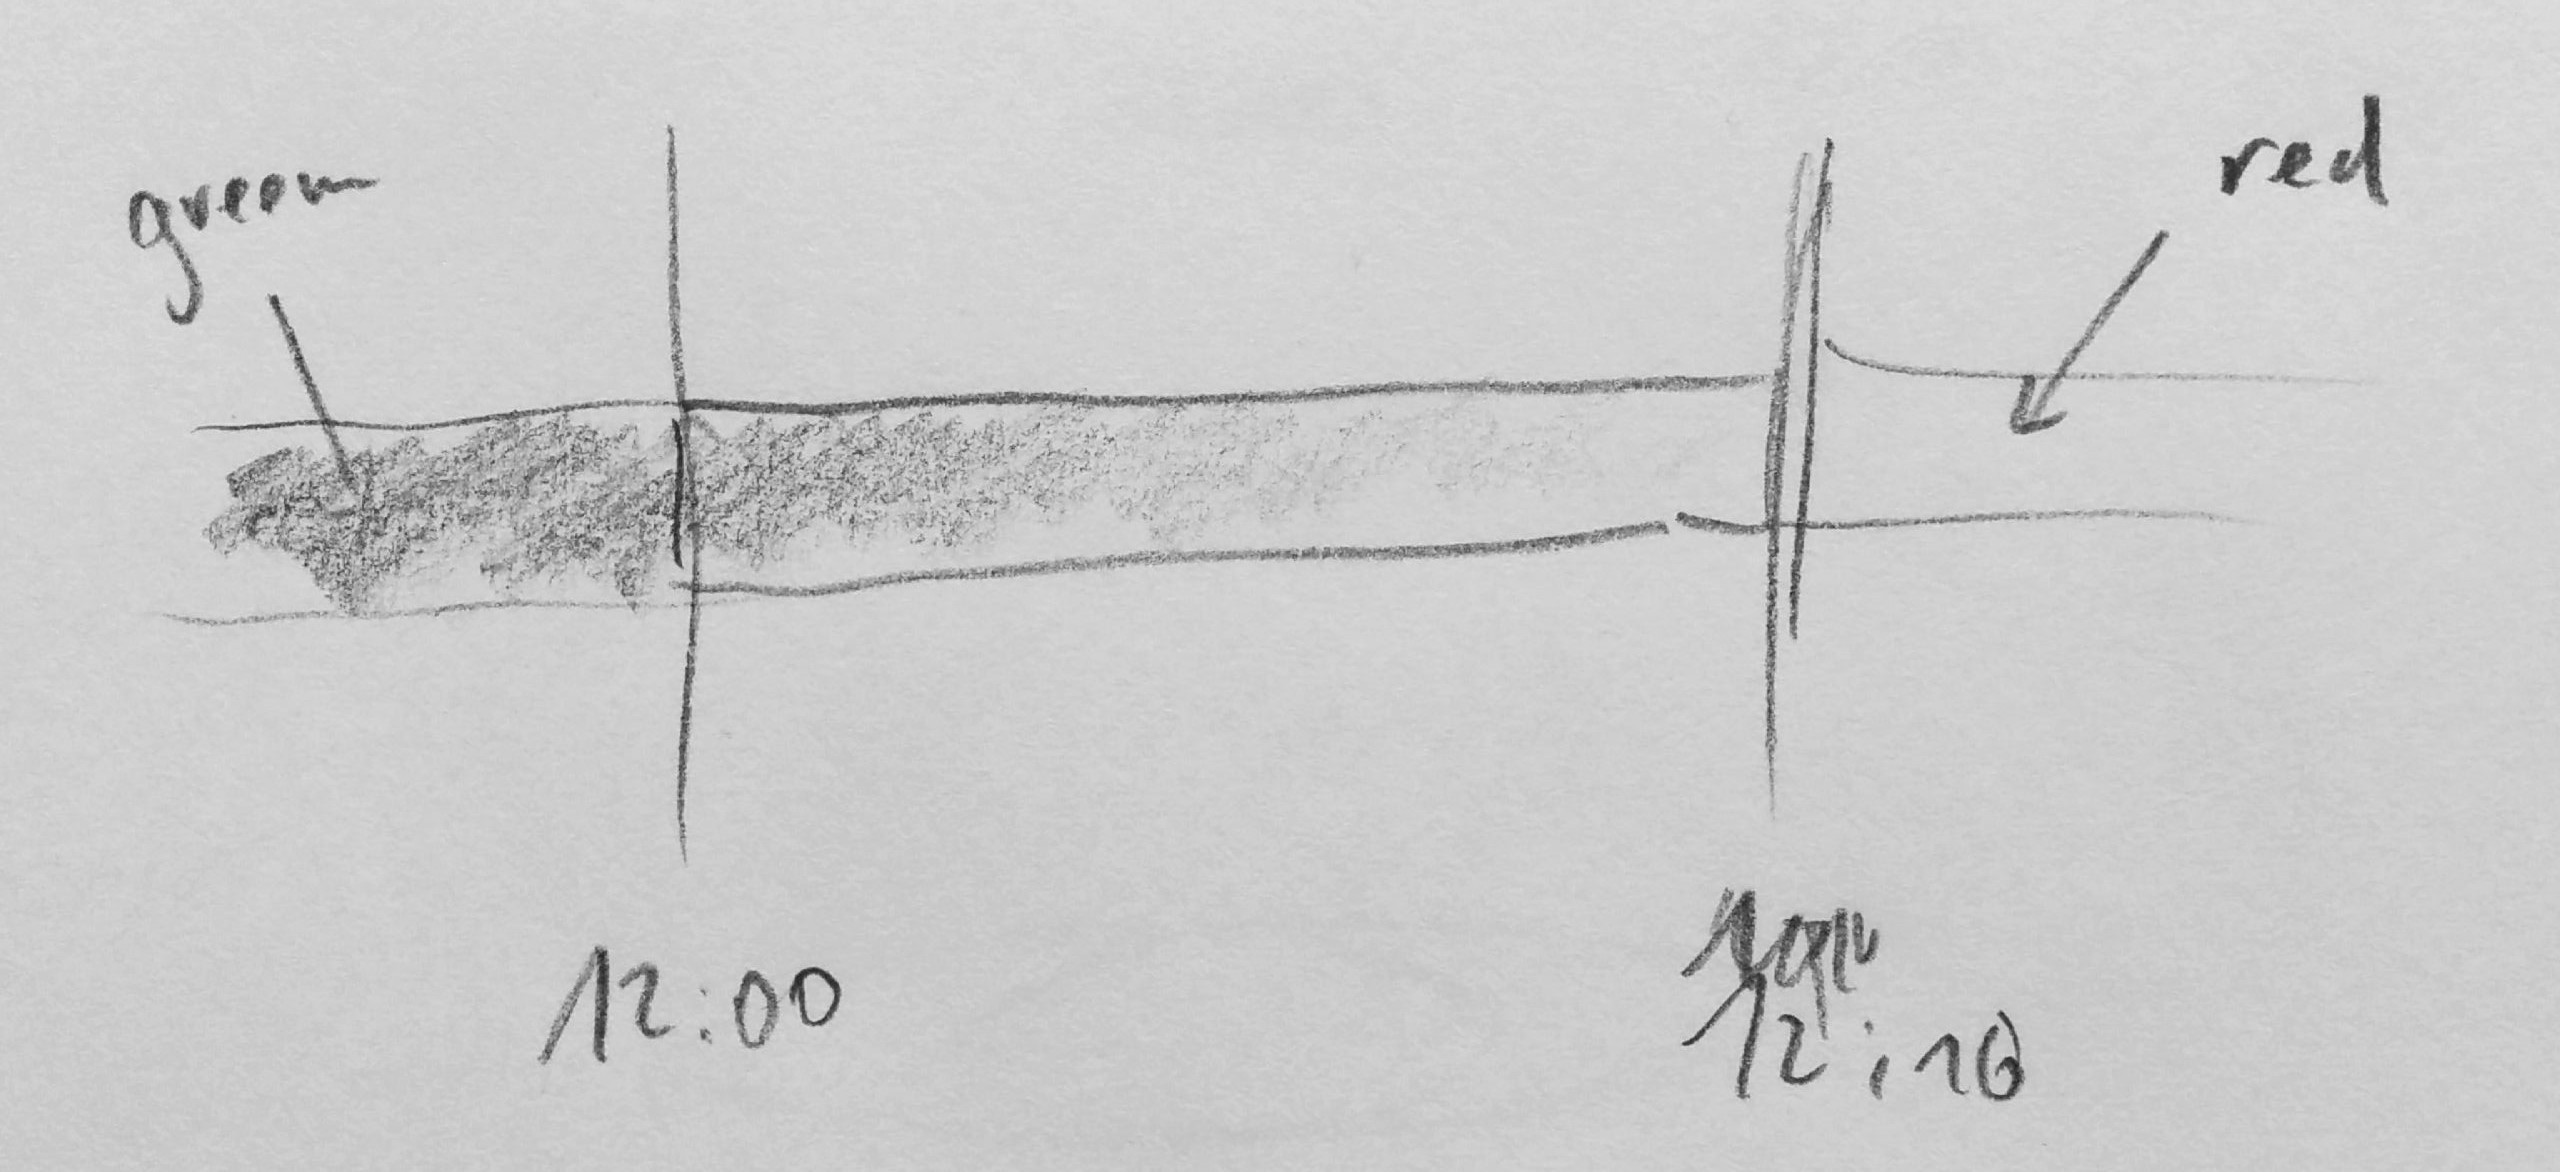
\includegraphics[height=0.5\textwidth]{figures/gradientSketch.jpg}
		\caption{\textit{This sketch utilizes a color gradient from green to red to represent the probability of a specific point in time.}}
		\label{fig:gradSketch}
	\end{minipage}
	\begin{minipage}{.55\textwidth}
		\centering
		\captionsetup{width=1.0\textwidth}
		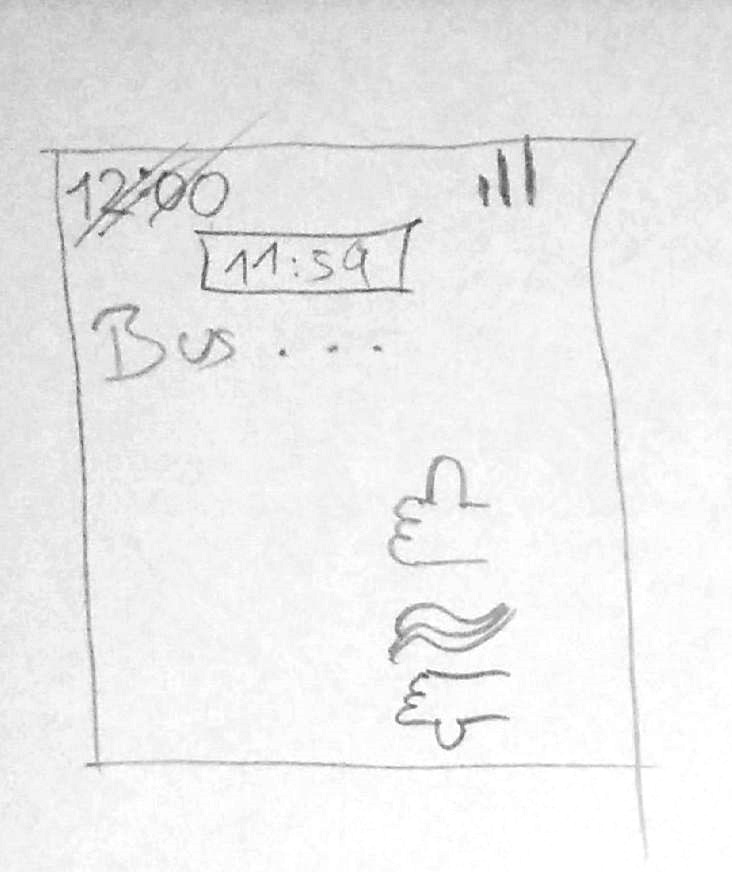
\includegraphics[height=0.55\textwidth]{figures/iconSketch.jpg}
		\caption{\textit{In this design the participant worked with user interaction and icon representations. The user has to enter a point in time and receives an icon, representing the corresponding probability, as feedback.}}
		\label{fig:iconSketch}
	\end{minipage}
\end{figure}

Other explicit representations of uncertainty utilize icons to convey the actual probability values to the user. An example for this can be seen in Figure \ref{fig:iconSketch}. We believe this approach to be especially intuitive, but lacks the precision to represent exact values. Therefore we think: \textbf{H3 Icon representations, like smiley faces, are a good approach to represent probability values in a very intuitive way, as long as these values do not have to be judged very precisely.}\par \medskip

Even though most visualizations feature an explicit representation of uncertainty, 11 sketches, like the one in Figure \ref{fig:bounded}, are of a bounded nature, which only shows the bounds of the uncertain interval, rather than explicit values. If this is the case because this is seemed to be the best way for these participants, or if they simply had no good idea to represent uncertainty explicitly, we do not know. Either way, these representations seem to be intuitive to most people, even though they are not well suited for the task at hand. \citet{gschwandtner2016visual} showed that this approach is well suited to convey durations and temporal bounds to the user, which leads us to the following joint hypothesis: \textbf{H4 Bounded visualizations are intuitive and effective ways to convey durations and temporal bounds of events with uncertain start and end times to non-expert users.}\par \medskip

\begin{figure}[H]
	\begin{minipage}{.5\textwidth}
		\centering
		\captionsetup{width=0.8\textwidth}
		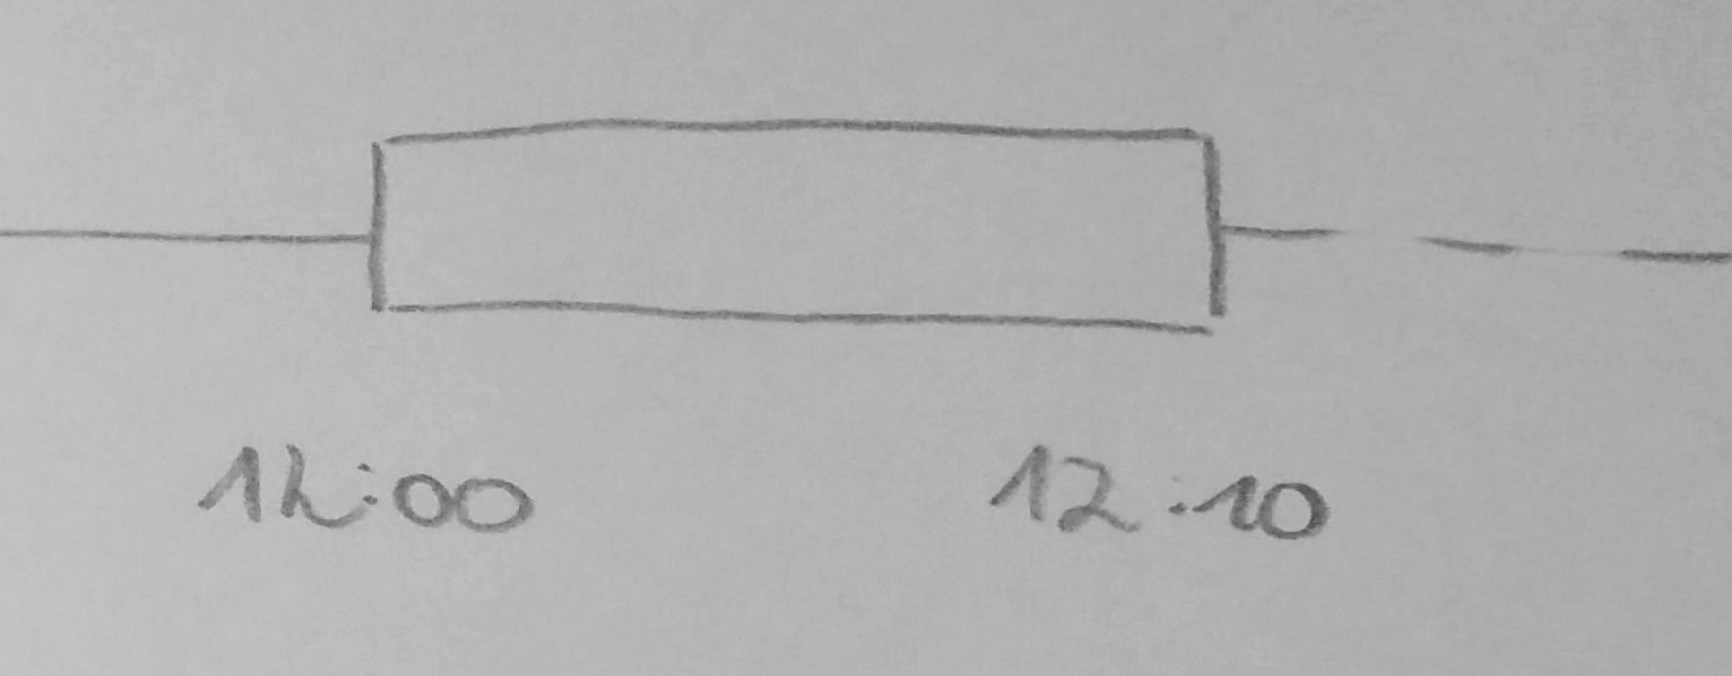
\includegraphics[height=0.35\textwidth]{figures/bounded.jpg}
		\caption{\textit{The broader part from 12:00 to 12:10 marks the uncertain part of the event, while the continuous line on the left marks the certain part.}}
		\label{fig:bounded}
	\end{minipage}
	\begin{minipage}{.5\textwidth}
		\centering
		\captionsetup{width=1.0\textwidth}
		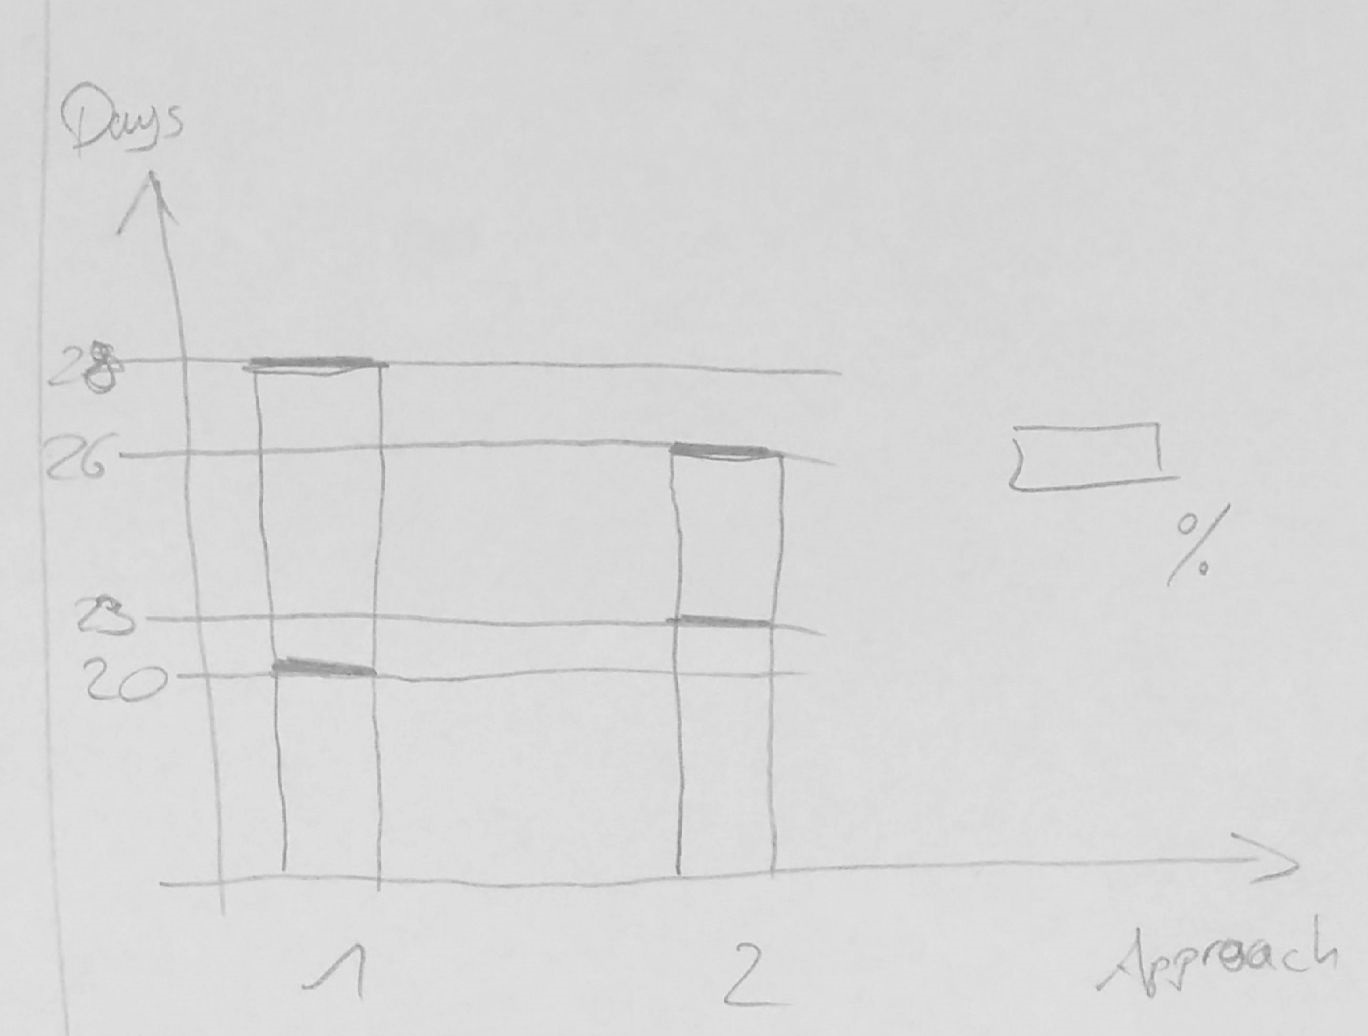
\includegraphics[height=0.6\textwidth]{figures/timeBotTop.jpg}
		\caption{\textit{In this vertical bar chart the time is mapped to the y-axis going from the bottom to the top. The two bars represent the two project approaches.}}
		\label{fig:timeBotTop}
	\end{minipage}
\end{figure}

\begin{figure}[H]
	\centering
	\captionsetup{width=0.8\textwidth}
	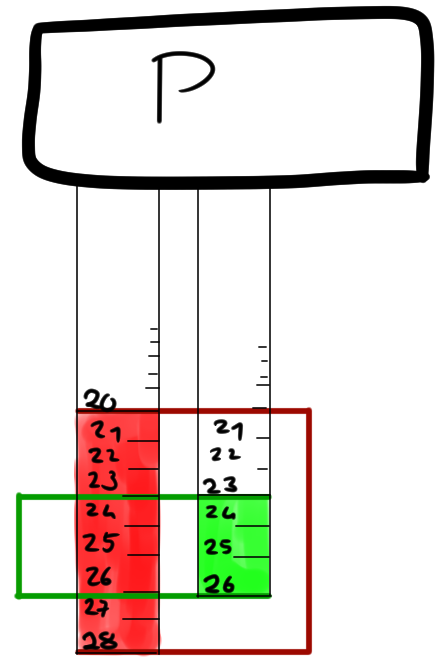
\includegraphics[height=0.45\textwidth]{figures/topbot.png}
	\caption{\textit{In this sketch the study participant elected to represent time in the horizontal axis from top to bottom, which is an uncommon approach within our study.}}
	\label{fig:topbot}
\end{figure}

The assumption that most people would represent time on the horizontal axis from left to right is confirmed by our results. See Figure \ref{fig:bounded} as an example. From the total amount of 93 sketches we collected and analyzed, 80\% represented time in this way. We also assumed that time would usually be represented from top to bottom, if the time line occupies the vertical axis. This assumption was falsified, since only two sketches featured time this way. One of them can be seen in Figure \ref{fig:topbot}. The rest of the drawings showed time either in a clockwise manner (clock metaphors) or from bottom to top, like in Figure \ref{fig:timeBotTop}. These findings indicate that the question regarding the truth of the following hypothesis can not trivially be answered: \textbf{H5 It is more intuitive to a non-expert user group to vertically map time from the bottom to the top, than vice versa.}\par \medskip

In Table \ref{tb:t23} the results of the \textit{Project Scenario} can be seen. It shows that only five drawings feature graph representations in the two encompassed tasks. One of them can be seen in Figure \ref{fig:compgraph}. We believe that this is due to the task we asked our participants to solve with their visualization. To judge the average time an event takes, people seem to prefer to see the two uncertain intervals next to each other, instead of superimposed graphs. \textbf{H6 If two or more events are compared to each other, it is more intuitive to show them in a juxtaposition, than superimposed in the same space.} This hypothesis is also supported by the numbers of superpositions (7) and juxtapositions (23) in the collected drawings. \par \medskip

\begin{figure}[H]
	\centering
	\captionsetup{width=0.8\textwidth}
	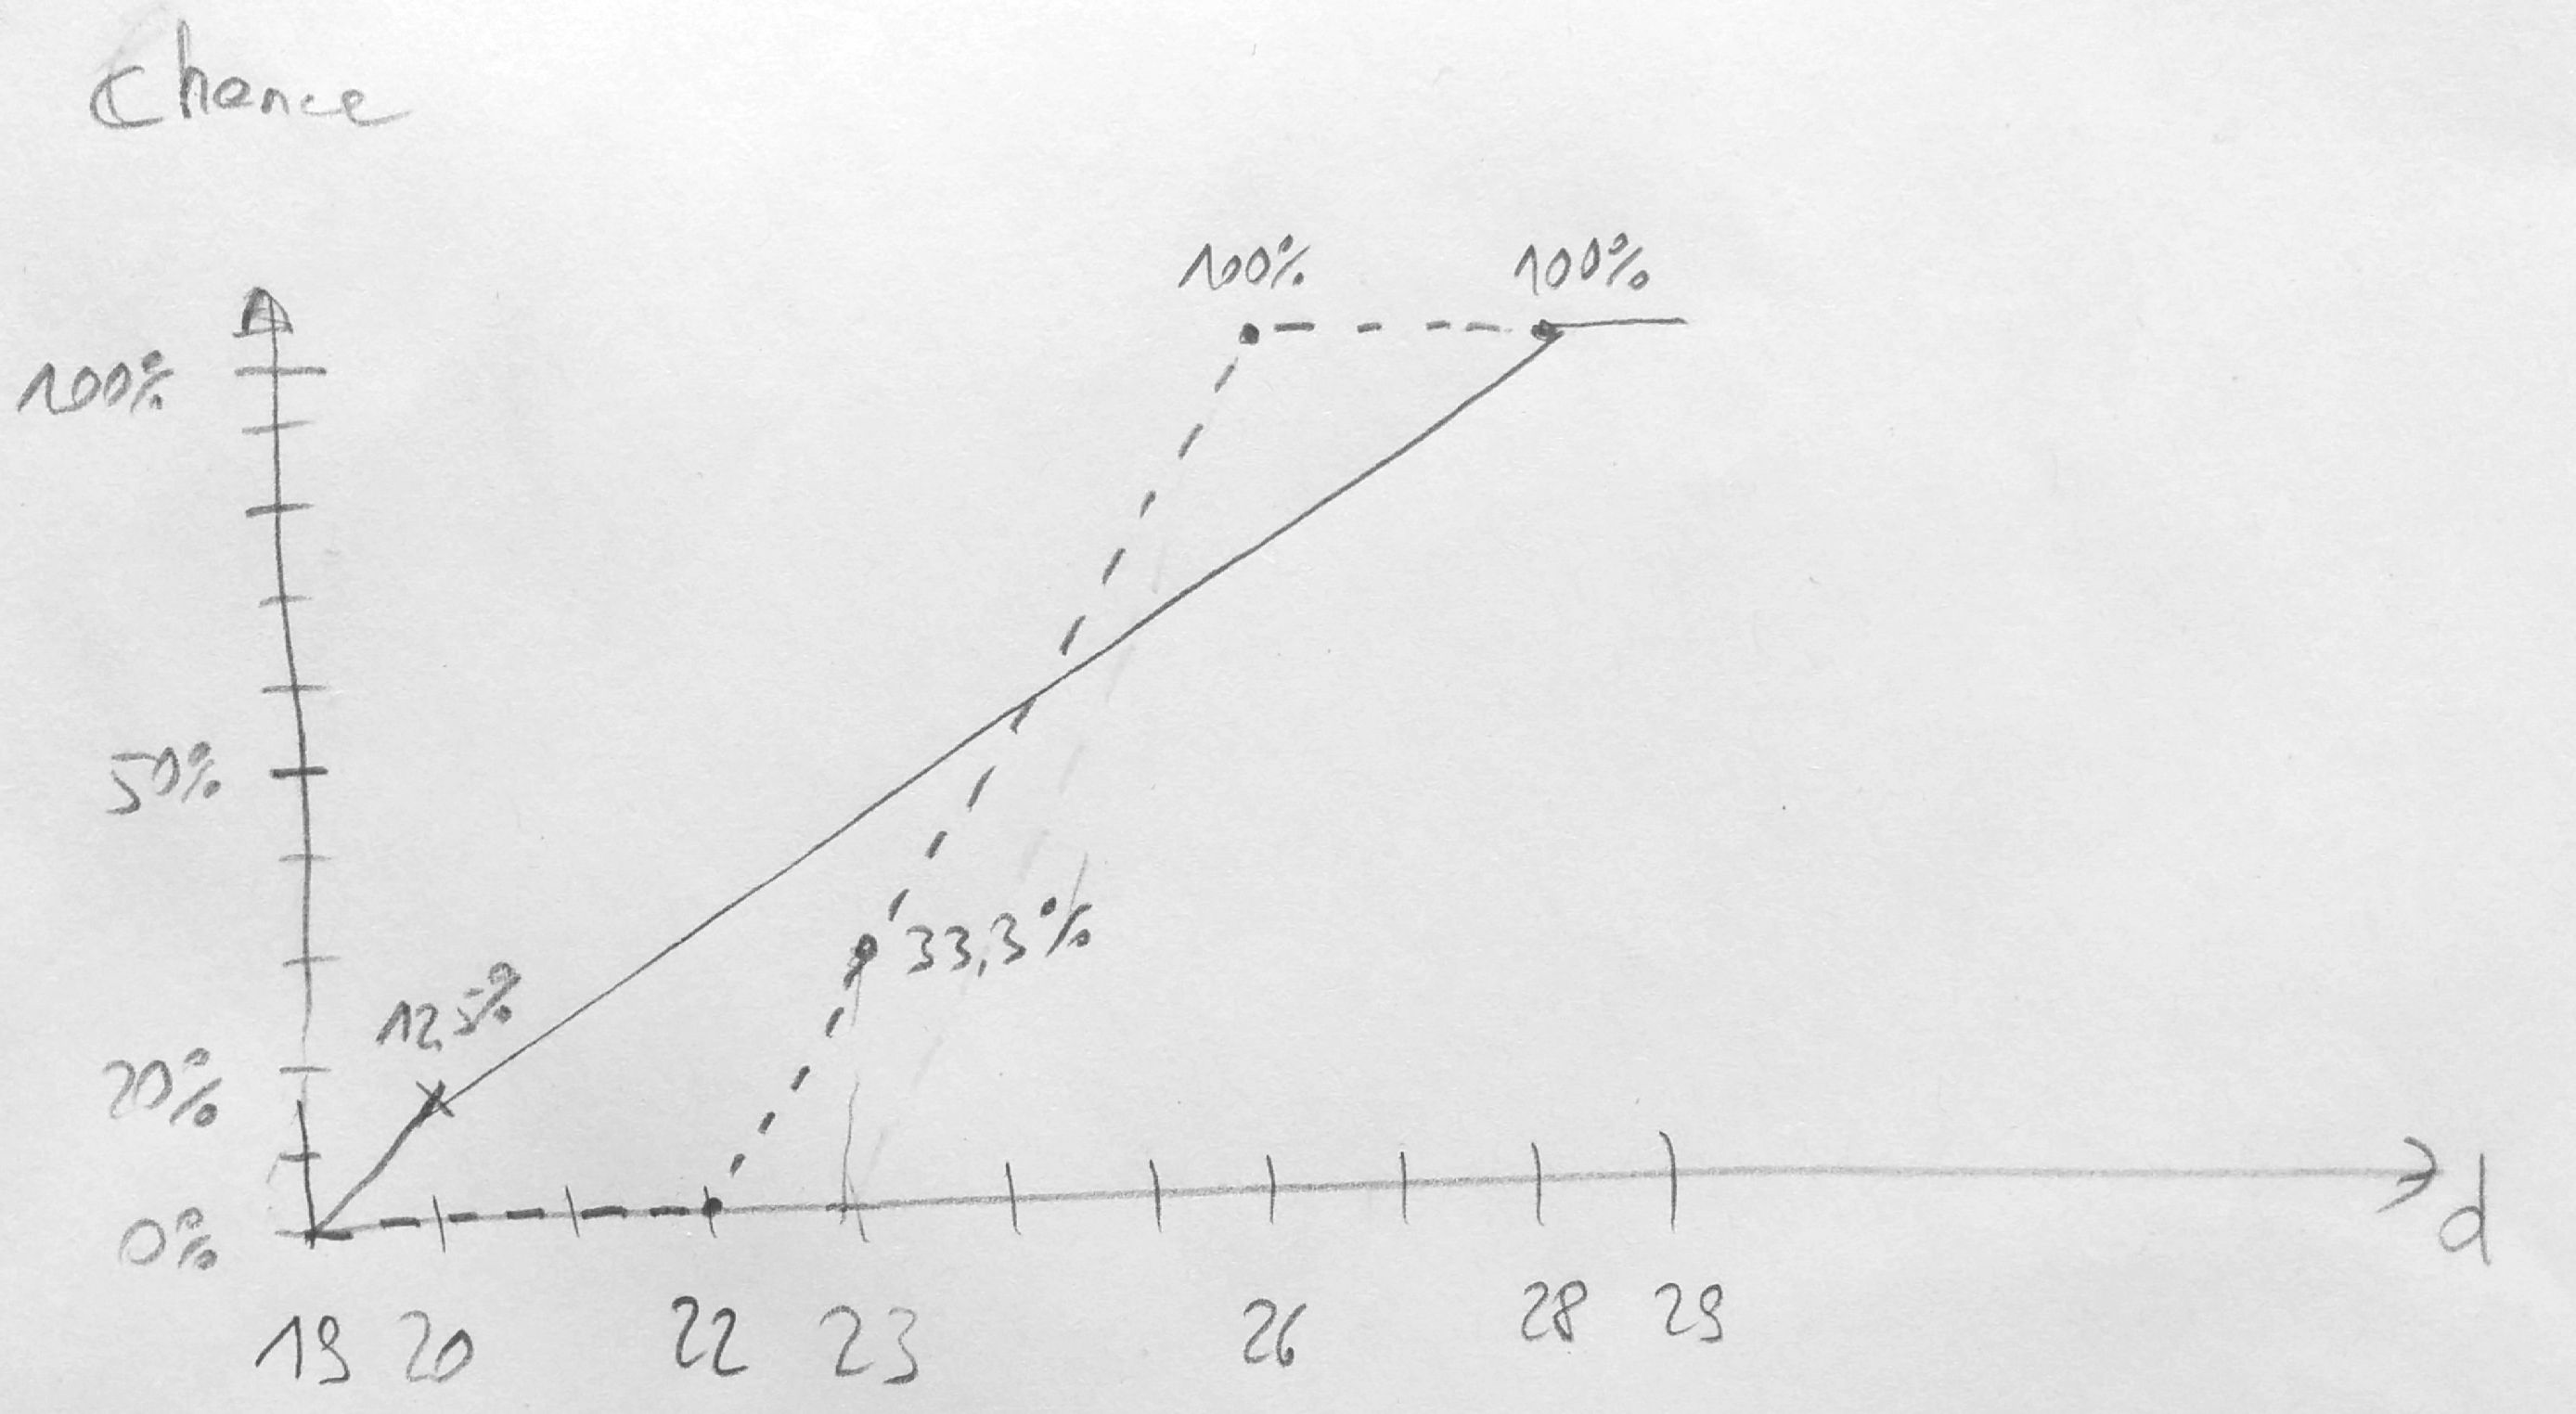
\includegraphics[height=0.45\textwidth]{figures/compgraph.jpg}
	\caption{\textit{This is one of the five sketches, which feature a graph representation to visualize the Project Scenario.}}
	\label{fig:compgraph}
\end{figure}

Another thing that can be seen in the results table of the \textit{Project Scenario}, is that most sketches feature an explicit representation of uncertainty, but there does not seem to be one favorite way to do so. Within the collected drawings uncertainty is represented using graphs (see Figure \ref{fig:t2graph}), other representations that encoded it in length or height (see Figure \ref{fig:t2length}), through color (see Figure \ref{fig:t2color}) and through interaction (see Figure \ref{fig:t2interaction}). All of those approaches came up five times within our experiment. Hence, the results do not show any indication of one of those techniques being more intuitive than others in the context of a comparative visualization. What can be seen though, is that there was not a single icon representation used for these tasks. We believe that the reason for this is that icons do not lend themselves to comparisons, since they also do not represent single values accurately. \textbf{H7 Icon representations are not well suited for direct comparison.} \par \medskip


\begin{figure}[H]
	\begin{minipage}{.5\textwidth}
		\centering
		\captionsetup{width=0.8\textwidth}
		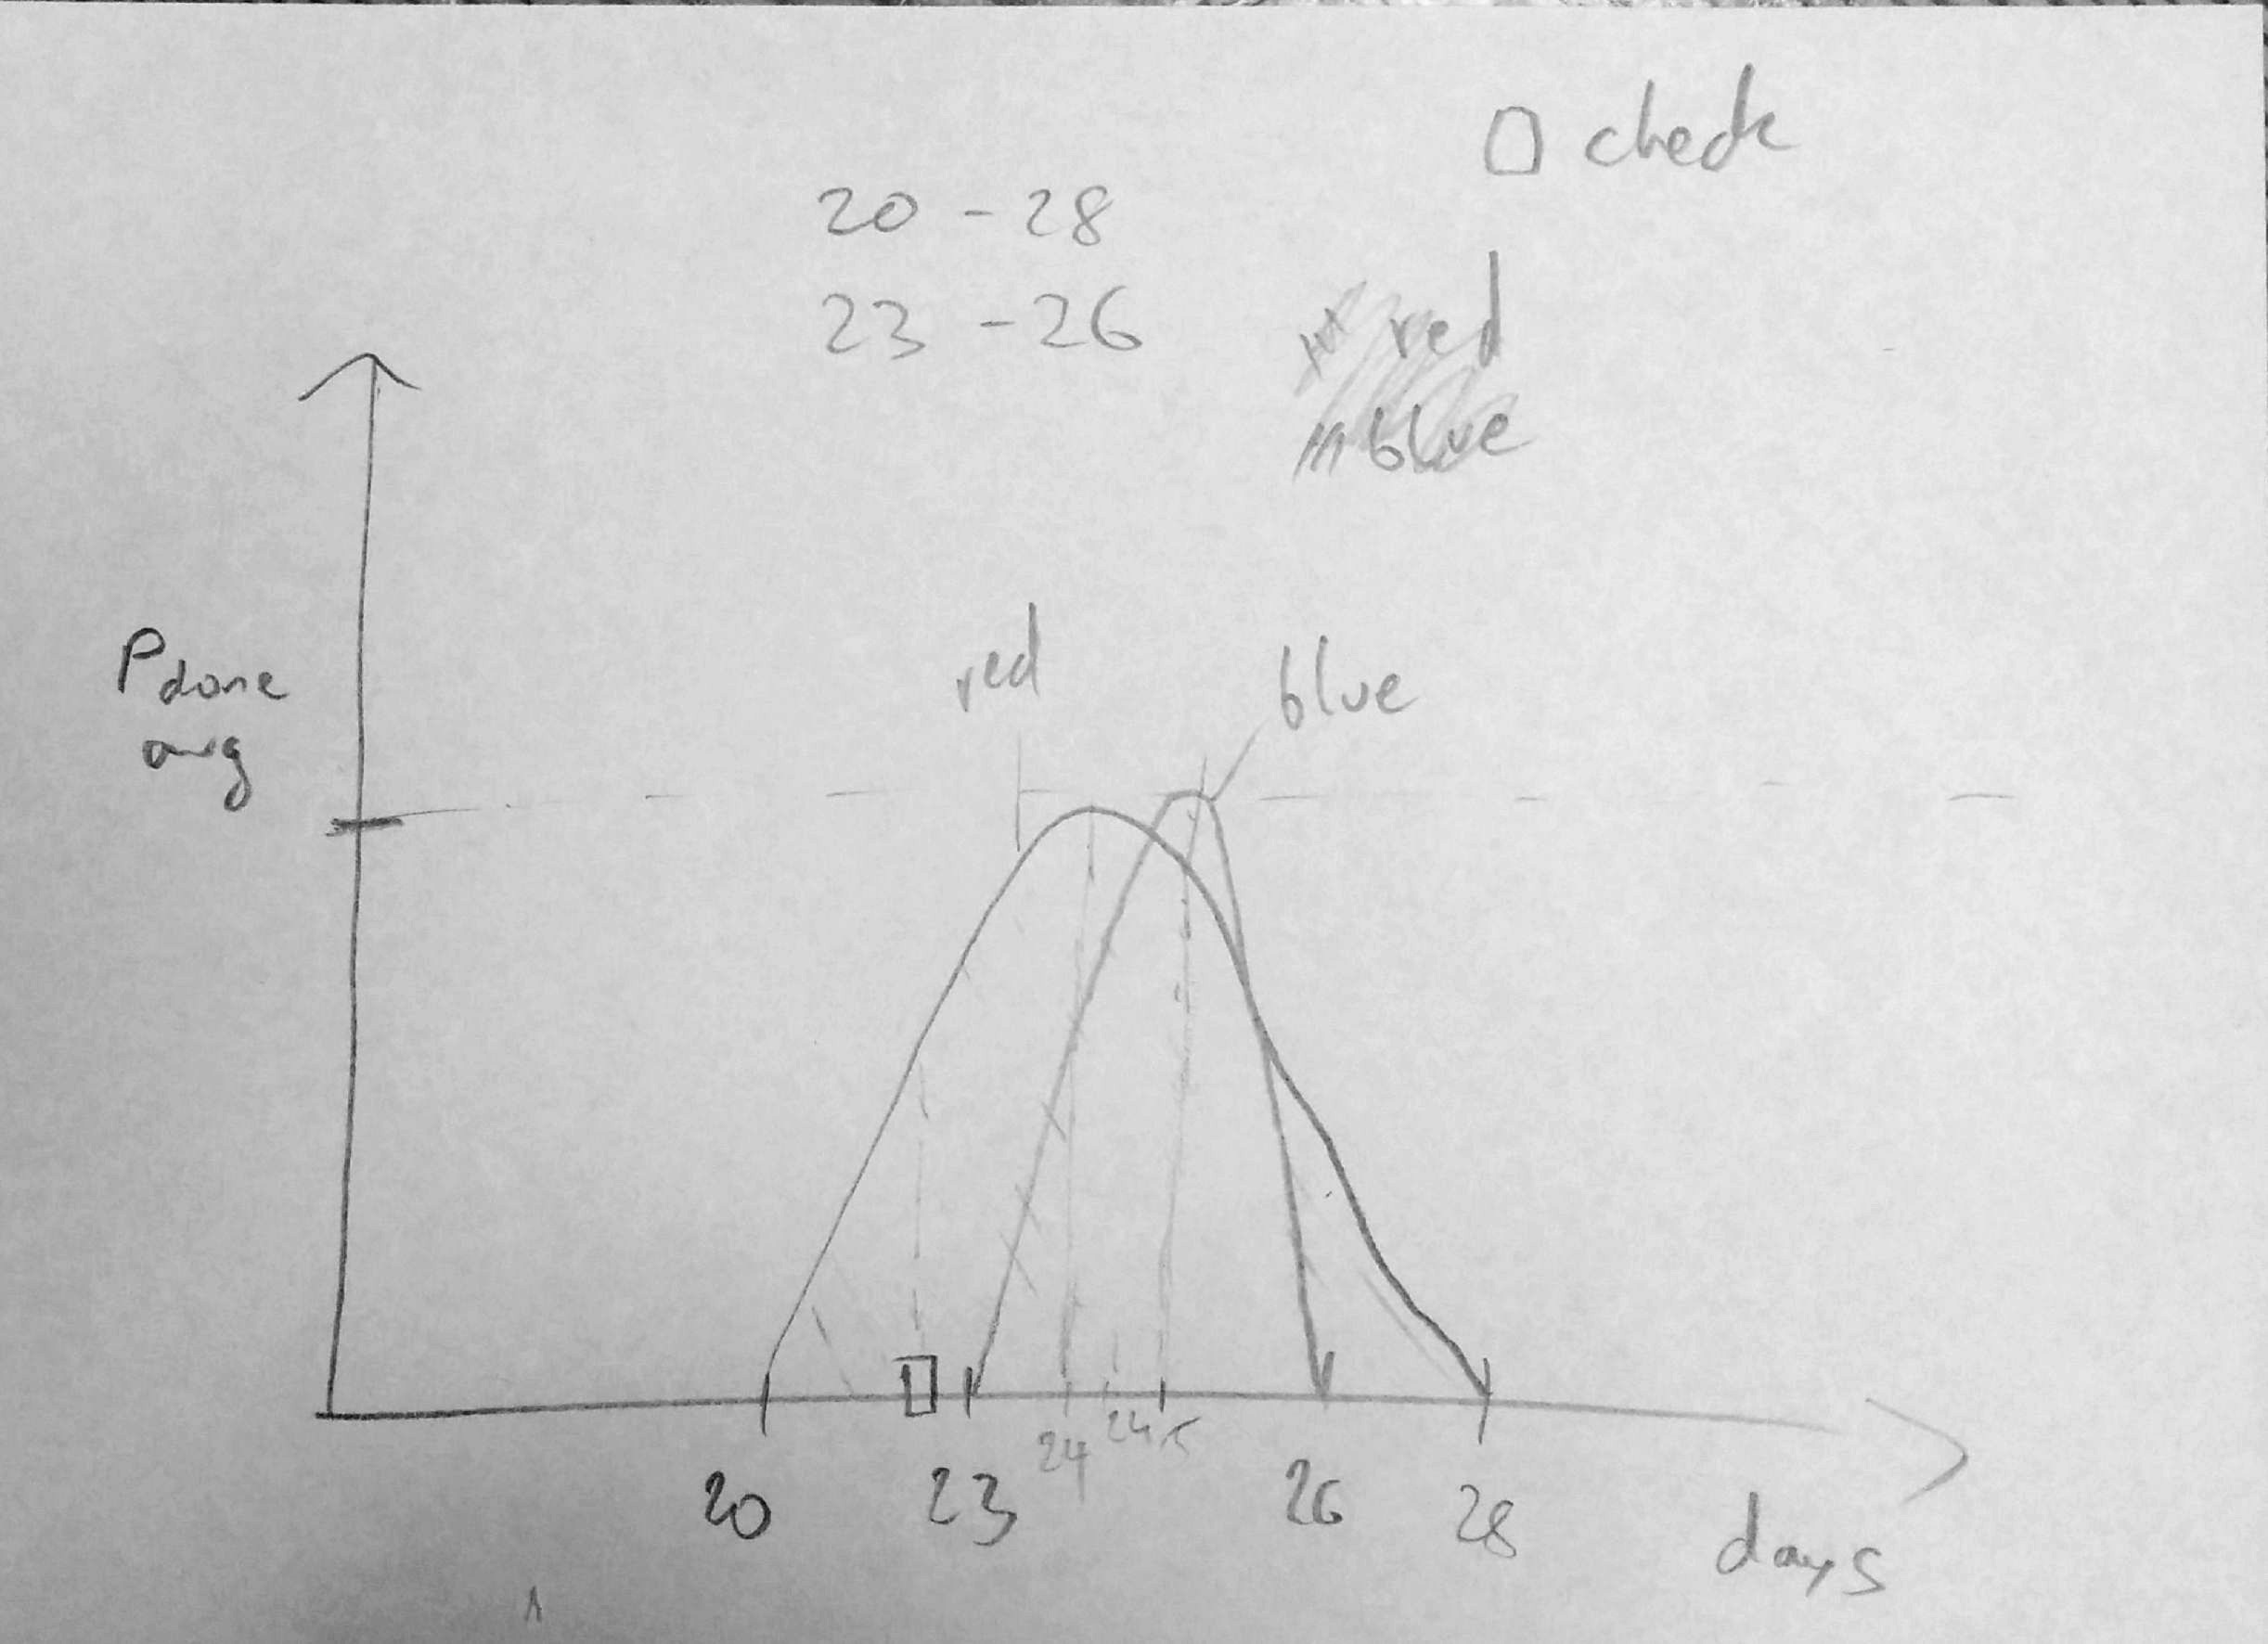
\includegraphics[height=0.5\textwidth]{figures/t2graph.jpg}
		\caption{\textit{This is a conventional graph visualization, that features two superimposed graphs. The graphs show the possibility of the event ending at the corresponding point in time.}}
		\label{fig:t2graph}
	\end{minipage}
	\begin{minipage}{.5\textwidth}
		\centering
		\captionsetup{width=1.0\textwidth}
		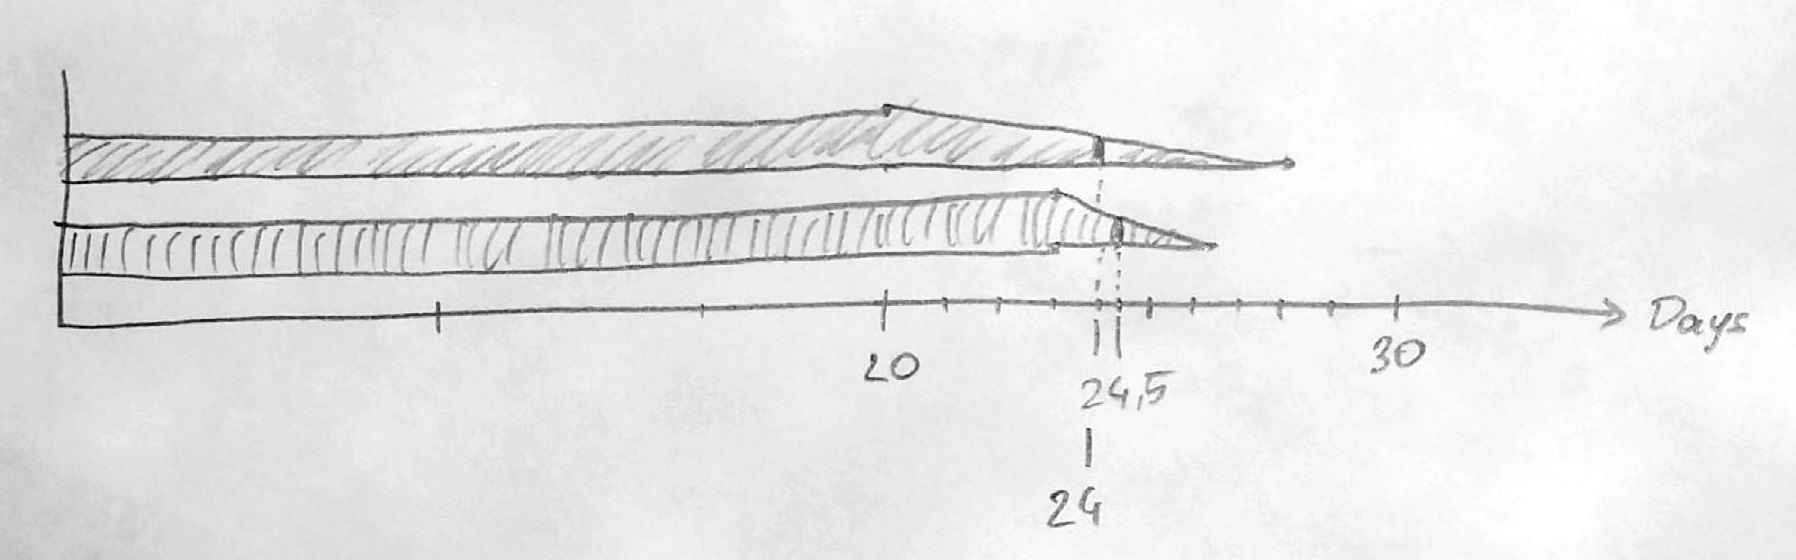
\includegraphics[height=0.33\textwidth]{figures/t2length.jpg}
		\caption{\textit{The uncertain time intervals are bounded by the sloping part of the horizontal bars. Additionally the thickness of the bar at a given point in time represents the possibility that the event is still going on at that point in time.}}
		\label{fig:t2length}
	\end{minipage}
\end{figure}
\begin{figure}[H]
	\begin{minipage}{.5\textwidth}
		\centering
		\captionsetup{width=0.8\textwidth}
		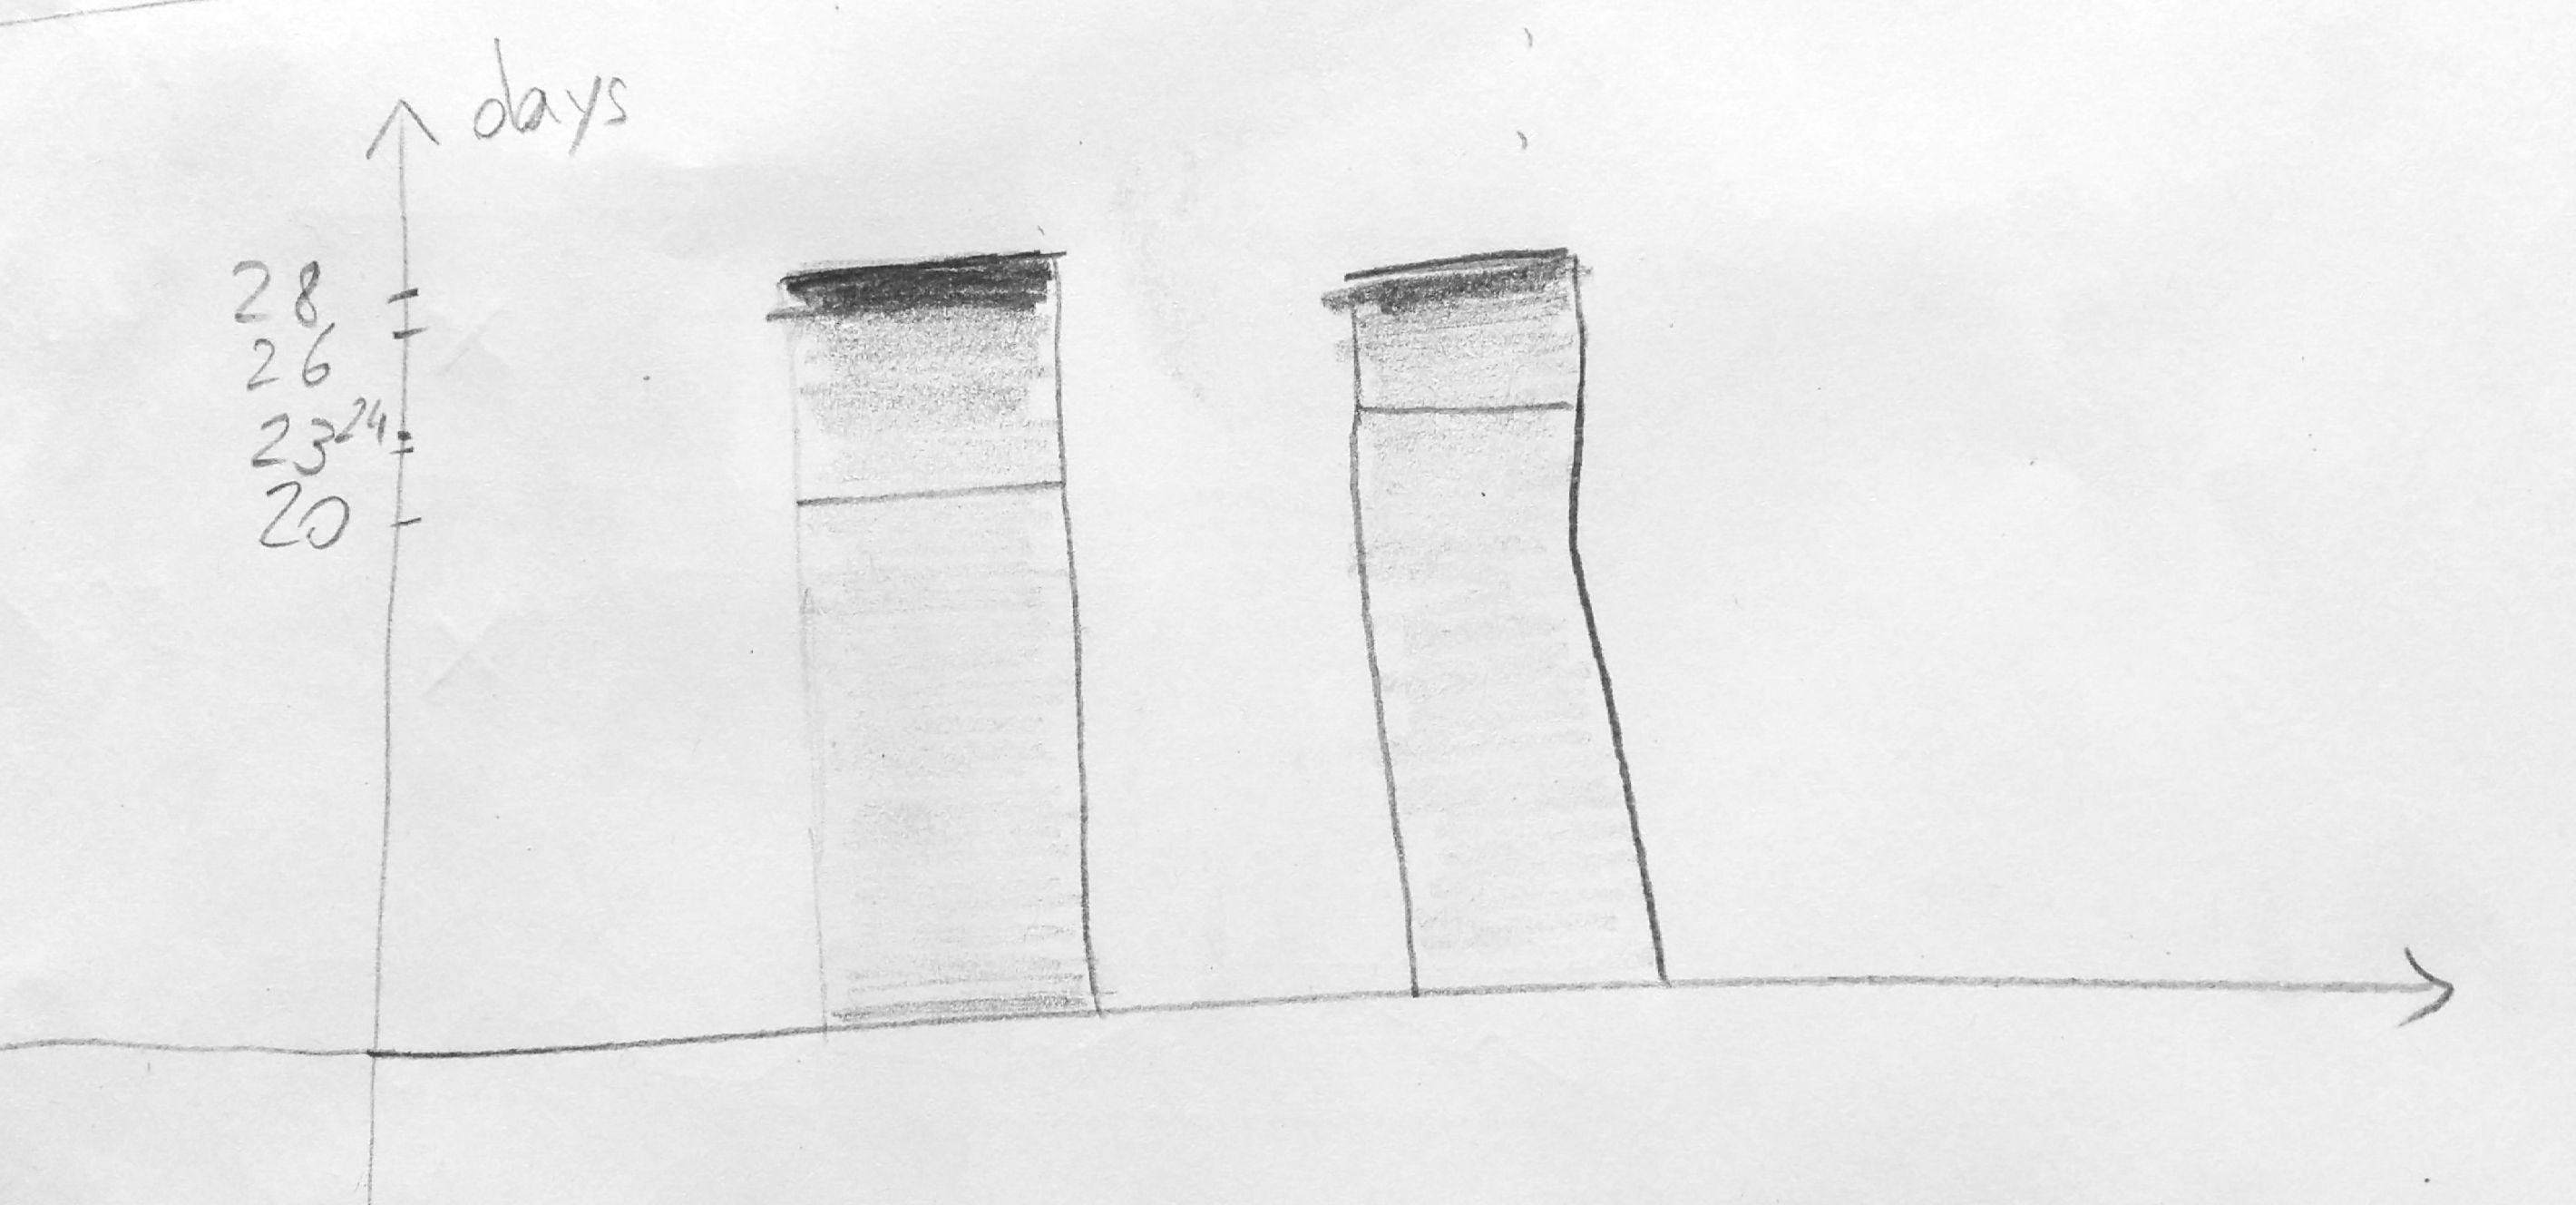
\includegraphics[height=0.4\textwidth]{figures/t2color.jpg}
		\caption{\textit{In this vertical bar chart color is used to additionally show the uncertainty explicitly for every point in time.}}
		\label{fig:t2color}
	\end{minipage}
	\begin{minipage}{.5\textwidth}
		\centering
		\captionsetup{width=1.0\textwidth}
		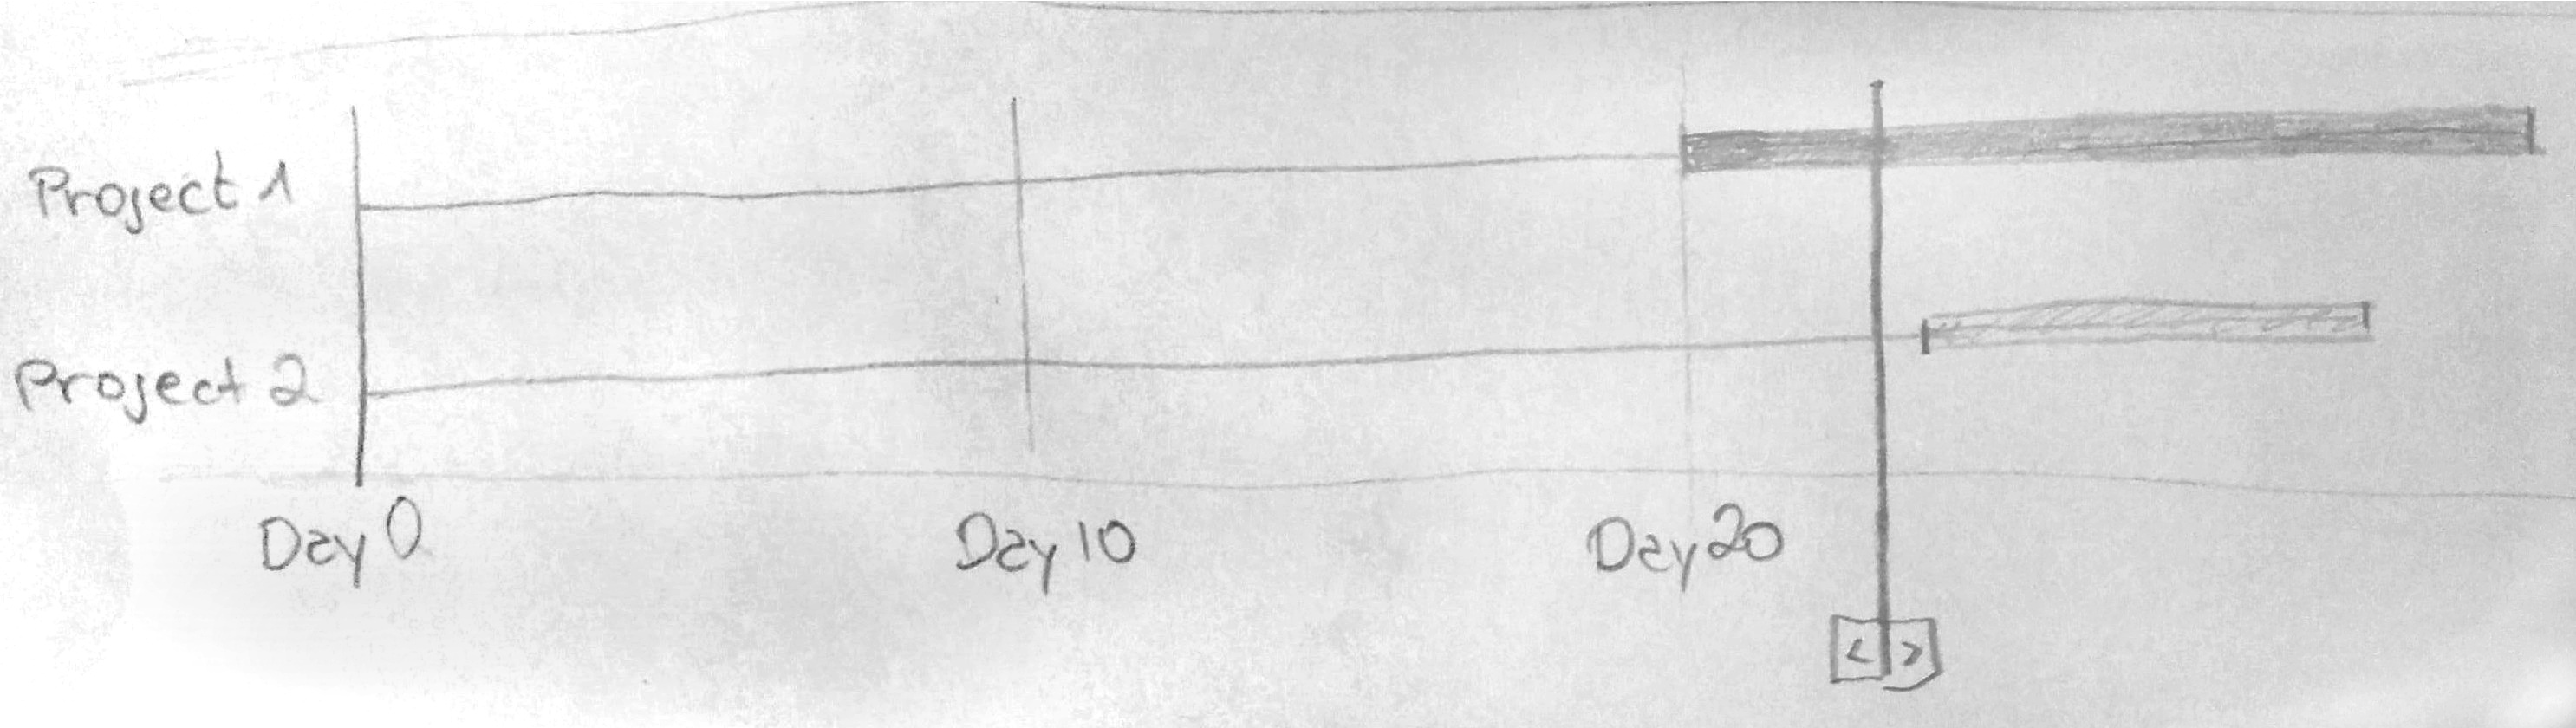
\includegraphics[height=0.3\textwidth]{figures/t2interaction.jpg}
		\caption{\textit{This visualization only shows the bounds of the uncertain time frames, but also shows explicit values through user interaction. The user can slide the slider on the bottom to a specific time point to get information about the respective possibilities of both events.}}
		\label{fig:t2interaction}
	\end{minipage}
\end{figure}


Even though most sketches feature uncertainty in an explicit way, there are still many bounded visualizations. We believe that this is due to our task description. To support the user in the first goal of the \textit{Project Scenario}, only the average value of the two intervals are needed. Hence, there is no need to visualize uncertainty to a given point in time explicitly. The fact that uncertainty was drawn so many times, even though it is not relevant for the task at hand, might be an indication that: \textbf{H8 Most people prefer to have the underlying uncertainty of data presented to them, even if it is not directly relevant for the task at hand.} An example for the additional visualization of uncertainty can be seen in Figure \ref{fig:t2length}.  \par \medskip

Table \ref{tb:t4} shows the results of the \textit{Lecture Scenario}. The most apparent difference between these results and the previous ones is that over two thirds of sketches feature the two relevant time intervals in a superimposed view (see Figure \ref{fig:t4clock}), instead of a juxtaposition (see Figure \ref{fig:t4bounded}). We believe that this is due to the nature of the task. In contrast to the previous scenario, the two intervals are both happening after each other, with the possibility of overlap and there is not direct comparison of the two. \textbf{H9 To represent the amount of overlap between events, it is intuitive to superimpose them in the same view.}\par \medskip

It is also noteworthy that there are more clock metaphors, like the one in Figure \ref{fig:t4clock}, used in this task, compared to the previous ones. We believe that this is because: \textbf{H10 Clocks lend themselves to show two superimposed time intervals, as long as the overlapping area does not exceed a one hour time frame.} \par \medskip

\begin{figure}[H]
	\begin{minipage}{.5\textwidth}
		\centering
		\captionsetup{width=0.8\textwidth}
		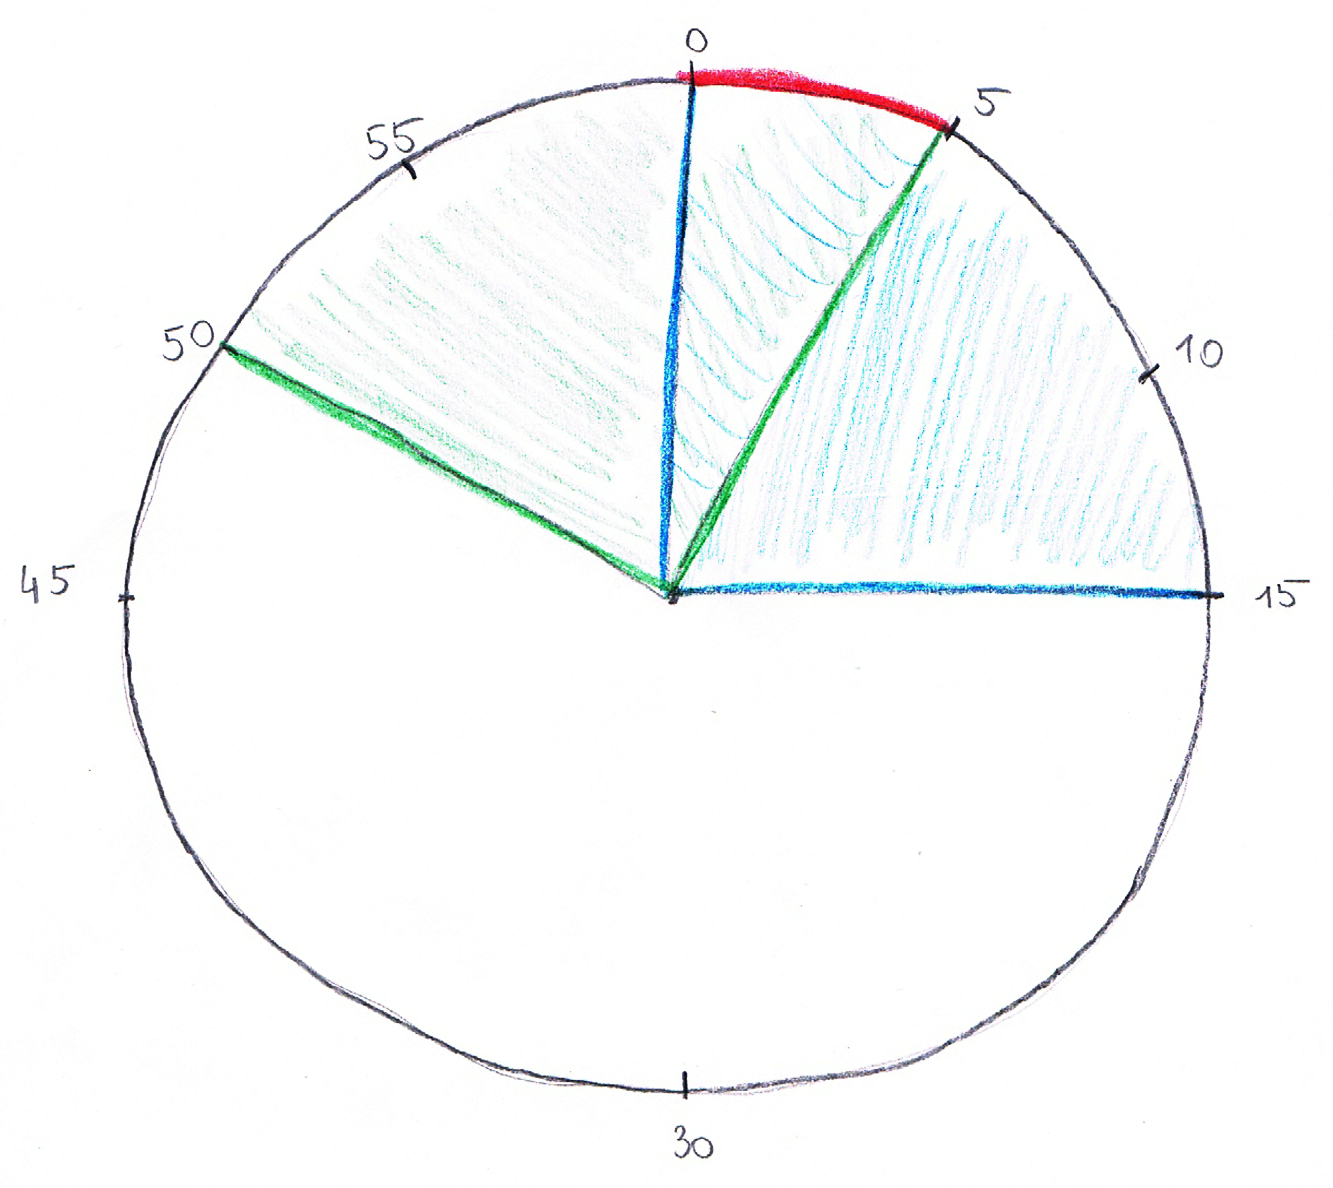
\includegraphics[height=0.6\textwidth]{figures/t4clock.png}
		\caption{\textit{This sketch shows a simple bounded clock visualization. Both uncertainty intervals are colored wedges on the clock. The two colors are mixed within the overlap of the two intervals.}}
		\label{fig:t4clock}
	\end{minipage}
	\begin{minipage}{.5\textwidth}
		\centering
		\captionsetup{width=1.0\textwidth}
		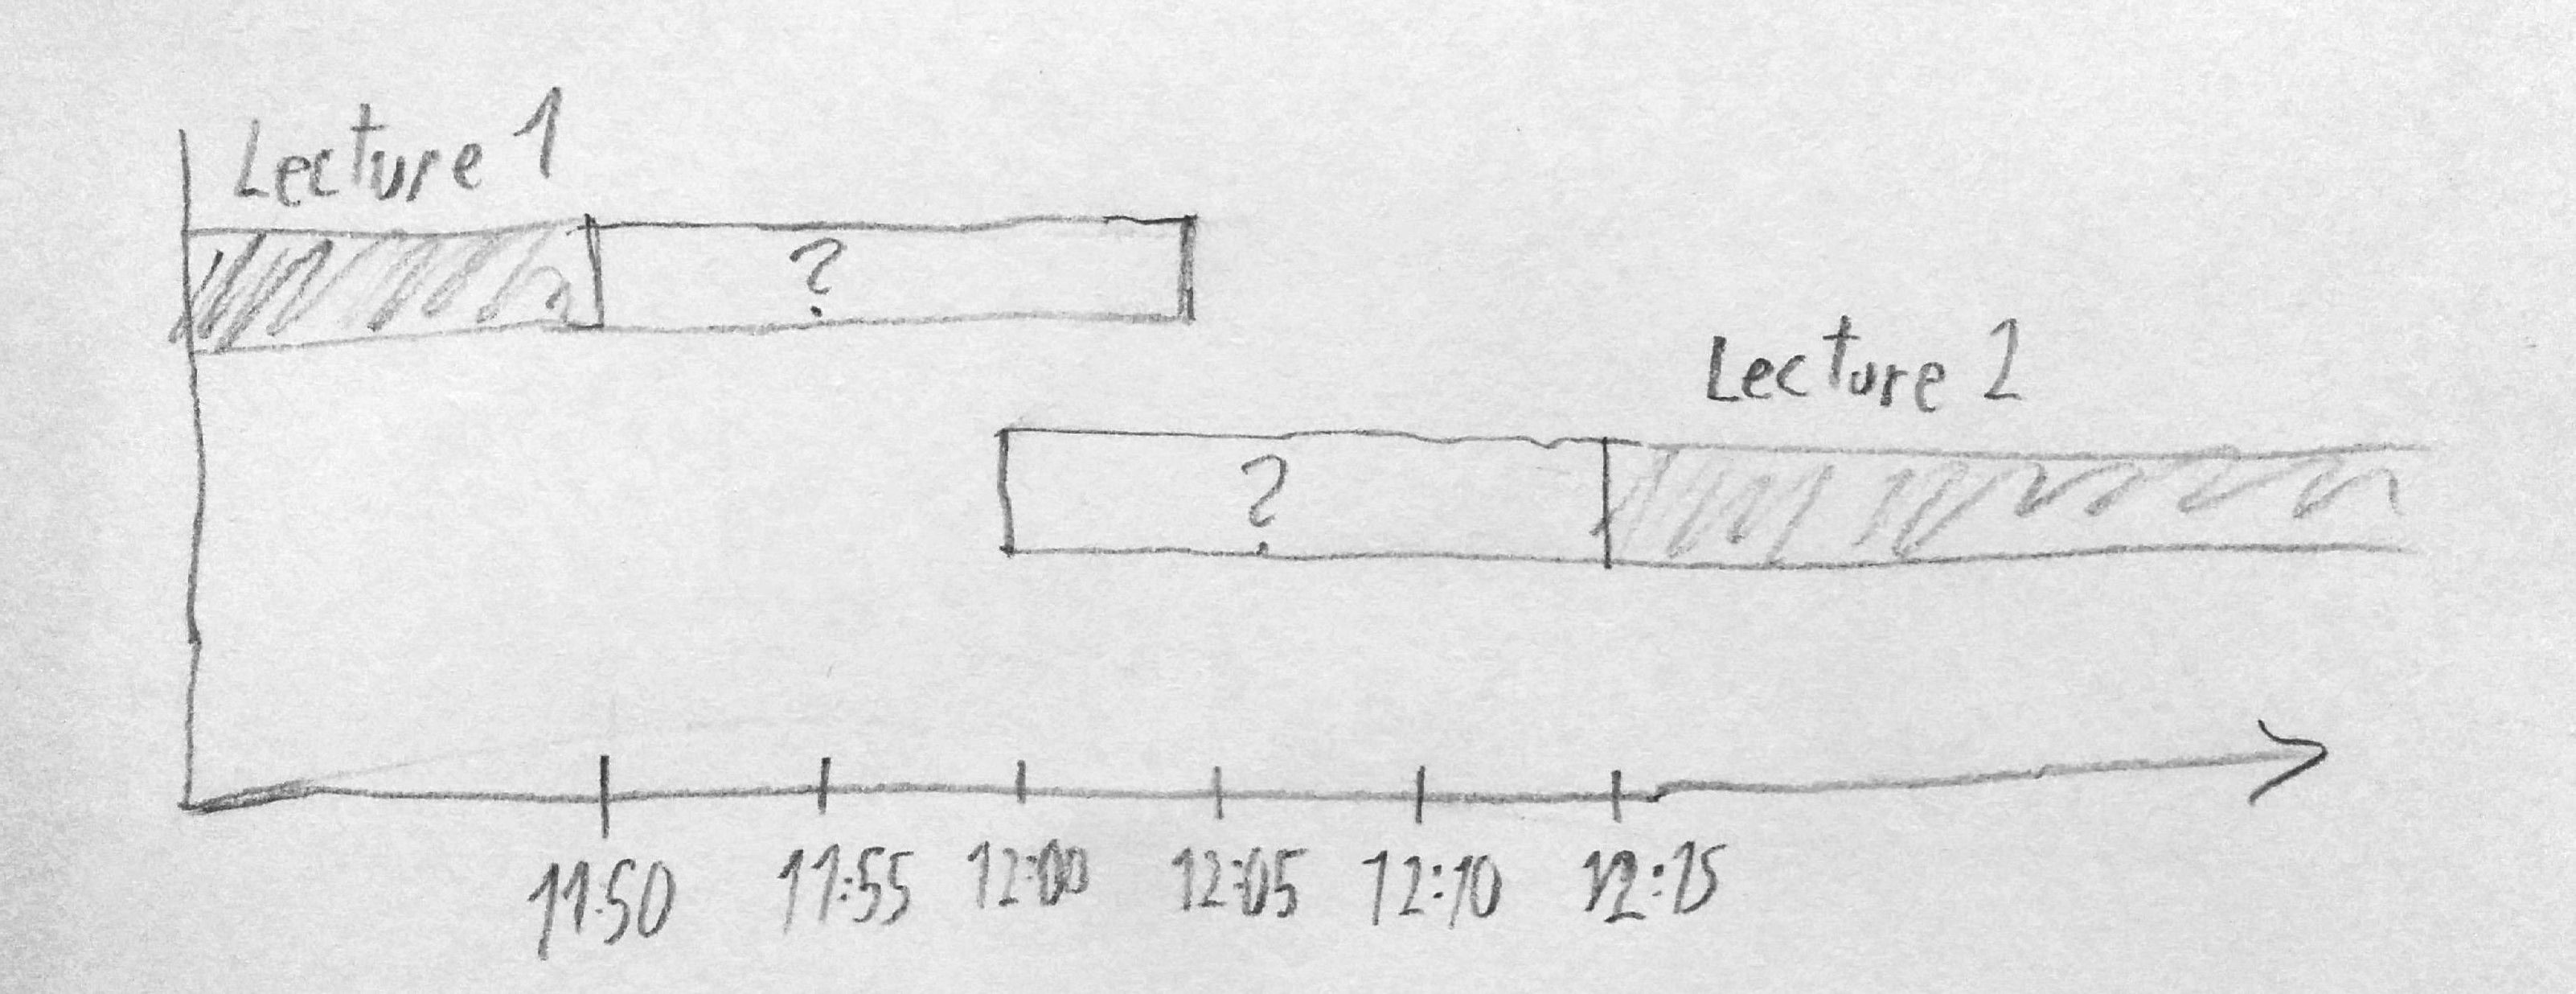
\includegraphics[height=0.4\textwidth]{figures/t4bounded.jpg}
		\caption{\textit{In this sketch both uncertainty intervals are only given by their temporal bounds. The user is not directly supported in figuring out what the possibility of overlap of the two events is.}}
		\label{fig:t4bounded}
	\end{minipage}
\end{figure}

Another significant difference to the last scenario is the lower amount of explicit uncertainty representations. About two thirds of all sketches of the \textit{Lecture Scenario} are bounded ones, like the one in Figure \ref{fig:t4bounded}. We believe that this is due to the complexity of the underlying goal. It is not trivial to visualize the joint probability of overlap of two intervals. Hence, most people do not have a good idea how to do it and simply visualize the bounds of the two intervals. \textbf{H11 An elaborate way of visualizing the joint probability of two uncertain events, to represent their overlap possibility is not very intuitive for most people.} \par \medskip

Taking a closer look at the sketches that utilize a superposition of the two intervals, shows that half of them use color to distinguish the intervals from each other. An example for this can also be seen in Figure \ref{fig:t4clock}. The other half does not need color to distinguish them, since they are characterized by their shape or position, like in Figure \ref{fig:t4pos} and \ref{fig:t4shape}. \textbf{H12 Color is an intuitive way of separating two overlapping objects of the same shape.}\par \medskip

\begin{figure}[H]
	\begin{minipage}{.5\textwidth}
		\centering
		\captionsetup{width=0.8\textwidth}
		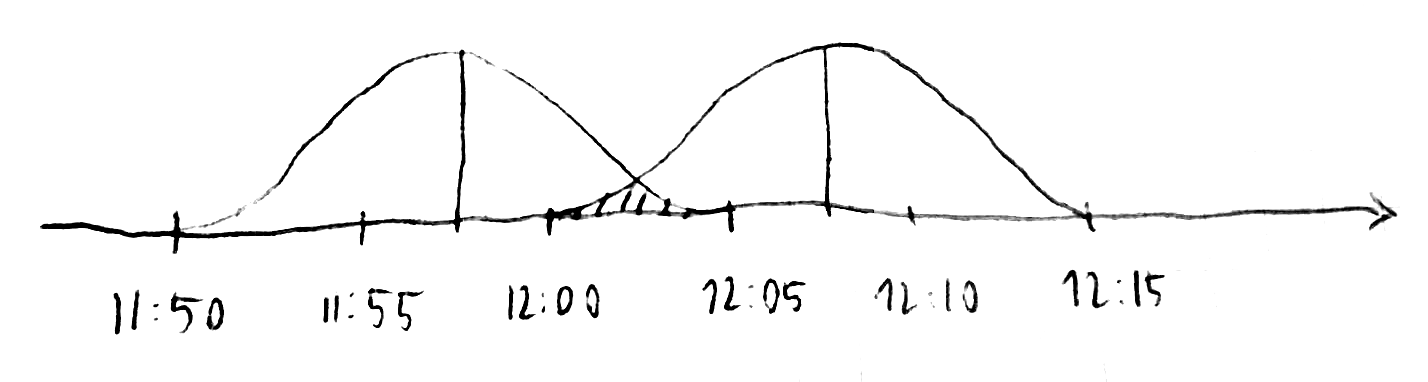
\includegraphics[height=0.28\textwidth]{figures/t4pos.png}
		\caption{\textit{The two graphs, which represent the respective uncertainty intervals of the two events, do not need to be distinguished by color, because they are separated by their position.}}
		\label{fig:t4pos}
	\end{minipage}
	\begin{minipage}{.5\textwidth}
		\centering
		\captionsetup{width=1.0\textwidth}
		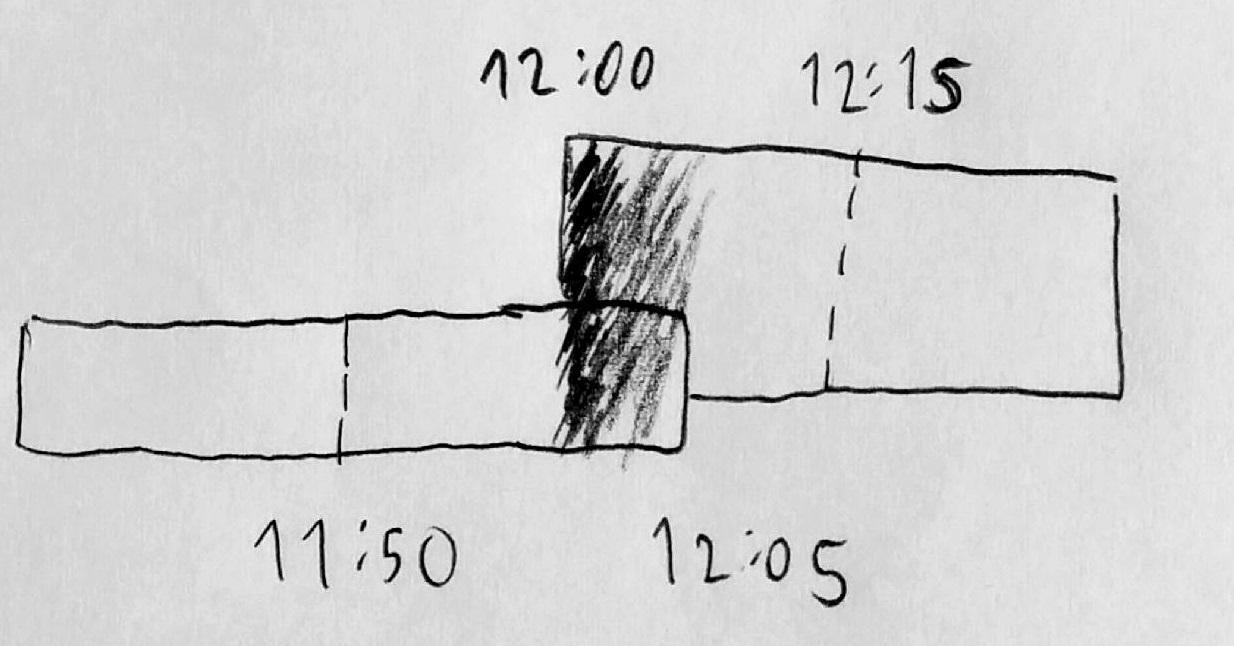
\includegraphics[height=0.45\textwidth]{figures/t4shape.jpg}
		\caption{\textit{In this case the participant used different shapes/sizes for the two uncertainty intervals, which left the color dimension to encode something else than the distinction between the two events.}}
		\label{fig:t4shape}
	\end{minipage}
\end{figure}


%%%%%%%%%%%%%%%%%%%%%%%%%%%%%%%%%%%%%%%%%

%%%%%%%%%%%%%%%%%%%%%%%%%%%%%%%%%%%%%%%%%
\chapter{Conclusion}
\label{ch:conclusion}
We conducted our \textit{Evaluation Study}, which is building on the work of \citet{gschwandtner2016visual}. Our goal was to evaluate for which kinds of tasks it makes sense to additionally visualize temporal uncertainty and for which tasks it does not bring any advantages. The study was conducted on three user groups, where each user group was supported by a different visualization type. The different visualization types were Gradient Plots, Ambiguation Plots and visualized mean values. Each group performed the same tasks, representing typical questions which might be asked when it comes to temporal uncertainties. Those tasks have been separated into four successive sessions. We defined three hypotheses which we wanted to verify by this user study. For evaluation of the gathered results, we performed statistical p-value tests, in particular Kruskal-Wallis tests, and also visually investigated the data by using boxplots. \par \medskip

Unfortunately, our study results did not confirm our hypotheses with absolute confidence. While, we had to reject our first hypothesis, our second and third hypotheses can only be considered plausible. The main reason for this is that the amount of participants we asked is too low for a quantitative user study. Still, the results show a visible trend, suggesting that the second and third hypotheses could hold. In order to verify our assumptions, future work might be needed where a more elaborate and more extensive study is conducted. \par \medskip

%____________________________________________________________________

Additionally to our quantitative \textit{Evaluation Study} we conducted a exploratory study called the \textit{Drawing Study}. This study has the goal of gaining insights about the intuitiveness of visual encodings for temporal uncertainty. Since the study is of exploratory nature, we did not proof any hypotheses we posed beforehand, but rather generated possible hypotheses from the study results, which could be the focus of future research. During the study we asked the participants to think of possible visualizations for given scenarios and tasks, and sketch them. We collected these drawings and analyzed them with an open coding approach. This means that we looked for similarities and distinctive features and defined categories, in which we could classify the sketches. The respective count of every class is the basis for our analysis. \par \medskip

Through our analysis we generated 12 hypotheses, which can be found in Chapter \ref{ch:discussion}. Most of them are only vaguely supported by our results so far. Because of this it is important to address these in future work and test them through quantitative studies. Since most of the proposed hypotheses regard the intuitiveness of visual encodings in a certain context, we believe that even if they are proven to be true they do not hold much value on their own. The true value lies in the joint insights that can be generated from multiple hypotheses. An example for this is our hypothesis \textbf{H2 Gradient Plots are intuitive representations to support the user in judging a specific probability value of a given point in time.} The knowledge that this visualization technique is intuitive is not valuable on its own, but if we combine it with the study results of \citet{gschwandtner2016visual} that tell us that Gradient Plots are also well fit to support a certain task, we get valuable and deployable insights. \par \medskip
%%%%%%%%%%%%%%%%%%%%%%%%%%%%%%%%%%%%%%%%%



%%%% Only for overview, can be deleted in the end
%\chapter{possible papers}
%\label{ch:papers}
%\input{chapters/papers}


%%%%%%%%%%%%%%%%%%%%%%%%%%%%%%%%%%%%%%%%%
%%% BACKMATTER %%%%%%%%%%%%%%%%%%%%%%%%%%
%%%%%%%%%%%%%%%%%%%%%%%%%%%%%%%%%%%%%%%%%

\appendix

\bibliographystyle{apalike}
\bibliography{references}

\end{document}